\documentclass[a4paper, 11pt]{report}

\usepackage{amsmath}
\usepackage{mathpazo}
\usepackage{natbib}
\usepackage[margin=1in]{geometry}
\usepackage{graphicx}

\usepackage[english]{babel} %language selection
\selectlanguage{english}

\pagenumbering{arabic}

\usepackage{hyperref}
\hypersetup{colorlinks, 
           citecolor=black,
           filecolor=black,
           linkcolor=black,
           urlcolor=black,
           bookmarksopen=true,
           pdftex}

\newcommand{\emversion}{2.0.0-alpha}
\newcommand{\libembversion}{1.0.0-alpha}

\newcommand{\subtitle}{for Embroidermodder \emversion, libembroidery \libembversion and all related projects}

\title{The Embroidermodder Project\\{\small \subtitle}}
\author{The Embroidermodder Team}

\begin{document}

\maketitle

\vspace{5in}

{\small
\url{https://embroidermodder.org}

Copyright (c) 2013-2022 The EmbroiderModder Team
}

\pagebreak

\tableofcontents

\pagebreak

\section*{The Embroidermodder Team}

The authors of this project include all people who have contributed to the project, those that have given their details to appear in these credits follow. 
``The Embroidermodder Team'' refers to this list generally.

Their name is in bold, github login in monospace, roles in normal font and any quotes they gave are emphasized.

\begin{itemize}
\item \textbf{Jonathan Greig} \texttt{redteam316} Core Developer, Artwork, Documentation, Designs, Commands
\item \textbf{Josh Varga} \texttt{JoshVarga} Core Developer
\item \textbf{Jens Diemer} \texttt{jedie} Documentation
\item \textbf{Kim Howard} \texttt{turbokim} Bug Fixes
\item \textbf{Martin Schneider} \texttt{craftoid} Documentation
\item \textbf{Edward Greig} \texttt{Metallicow} Artwork, Bug Fixes, Commands \emph{"It is a sin to wear the band's shirt on concert night, Unless you buy it @t the show."}
\item \textbf{Sonia Entzinger} Translation
\item \textbf{SushiTee} \texttt{SushiTee} Bug Fixes
\item \textbf{Vathonie Lufh} \texttt{x2nie} Bug Fixes, Bindings
\item \textbf{Nina Paley} Designs
\item \textbf{Theodore Gray} Designs
\item \textbf{Jens-Wolfhard Schicke-Uffmann} \texttt{Drahflow} BugFixes
\item \textbf{Emmett Lauren Garlitz - Some Little Sandy Rd, Elkview, West by GOD Virginia} \texttt{Oll Em} \textit{I have a nice cherry chess-top(Glass). "But remember, I NEVER played on it."}
\item \textbf{Robin Swift} \texttt{robin-swift} Core Developer, Documentation
\end{itemize}

\chapter{Introduction}

\section{History}

\chapter{The Graphical User Interface: Embroidermodder \emversion}

(UNDER MAJOR RESTRUCTURING, PLEASE WAIT FOR VERSION 2)

\begin{verbatim}
![Build Linux/GNU Status](https://github.com/Embroidermodder/Embroidermodder/actions/workflows/build_linux_gnu.yml/badge.svg)
![Build Mac OS Status](https://github.com/Embroidermodder/Embroidermodder/actions/workflows/build_macos.yml/badge.svg)
![Build Windows Status](https://github.com/Embroidermodder/Embroidermodder/actions/workflows/build_windows.yml/badge.svg)

![Test Linux/GNU Status](https://github.com/Embroidermodder/Embroidermodder/actions/workflows/test_linux_gnu.yml/badge.svg)
![Test Mac OS Status](https://github.com/Embroidermodder/Embroidermodder/actions/workflows/test_macos.yml/badge.svg)
![Test Windows Status](https://github.com/Embroidermodder/Embroidermodder/actions/workflows/test_windows.yml/badge.svg)
\end{verbatim}

Embroidermodder is a free machine embroidery application.
The newest version, Embroidermodder 2 can:

\begin{itemize}
\item edit and create embroidery designs
\item estimate the amount of thread and machine time needed to stitch a design
\item convert embroidery files to a variety of formats
\item upscale or downscale designs
\item run on Windows, Mac and Linux
\end{itemize}

For more information, see [our website](http://embroidermodder.org).

Embroidermodder 2 is very much a work in progress since we're doing a ground
up rewrite to an interface in Python using the GUI toolkit Tk.
The reasoning for this is detailed in the issues tab.

For a more in-depth look at what we are developing read
the developer notes\footnote{link to dev notes section}.
This discusses recent changes in a less formal way than a
changelog (since this software is in
development) and covers what we are about to try.

To see what we're focussing on at the moment check this table.

\begin{tabular}{l l}
\textbf{Date} & \textbf{Event} \\
\hline
April-June 2022 & Finish the conversion to C/SDL2 \\
July-August 2022 & Finish all the targets in the Design, or assign them to 2.1. \\
September 2022 & Bugfixing, Testing, QA. libembroidery 1.0 will be released, then updates will slow down and the Embroidermodder 2 development version will be fixed to the API of this version. \\
October 2022 & Embroidermodder 2 is officially released.
\end{tabular}

\section{Build and Install}

\subsection{Desktop}

First you must install the dependencies which aren't compiled into the source:

\begin{itemize}
\item \texttt{git}
\item \texttt{cmake}
\item \texttt{SDL2}
\item \texttt{SDL2\_image}
\item \texttt{SDL2\_ttf}
\item A C compiler (we recommend \texttt{gcc} or \texttt{clang})
\end{itemize}

on Debian Linux/GNU use:

\begin{verbatim}
  $ sudo apt install git clang build-essential libsdl2-dev \
        libsdl2-images-dev libsdl2-ttf-dev
\end{verbatim}

If you can't find a good fit for your system (on Windows use the section below),
try compiling the included submodules with:

\begin{verbatim}
  $ bash build_deps.sh
\end{verbatim}

From here, on most sytems the command:

\begin{verbatim}
  $ bash build.sh
\end{verbatim}

will build the software. Currently this is the 2.0-alpha, which will have a build code of
some kind.

\section{Dependencies and Build}

\chapter{The Low Level API: Libembroidery \libembversion}

\chapter{The Command Line Interface: \texttt{embroider}}

\section{Usage}

\chapter{Plans}

\subsubsection{Windows Specific Advice}

This is one of many possible ways to build the software on Windows,
this section is to help people who've not got a build environment to start with.

\begin{enumerate}
\item Download and install MSYS2 (follow their instructions): https://www.msys2.org/
\item Boot "Mintty" from the Start menu.
\item Use the commands:

\begin{verbatim}
$ pacman -S gcc cmake git bash mingw-w64-SDL2 mingw-w64-SDL2_image mingw-w64-SDL2_ttf
$ git clone https://github.com/Embroidermodder/Embroidermodder
$ cd Embroidermodder
$ bash build.sh
\end{verbatim}
\end{enumerate}

\subsubsection Mobile

These are currently unsupported (see iMobileViewer and Mobileviewer for
iOS and Android respectively), but after the Desktop version is
released we'll work on them.

The Mobile version will share some of the UI and all of the backend,
so development of the Desktop version will help us make both.

\subsection{Documentation}

The documentation is in the form of the website (included in the `docs/`
directory) and the printed docs in the three files:

\begin{itemize}
\item docs/libembroidery\_0.1\_manual.pdf
\item docs/embroidermodder\_1.90.0\_user\_manual.pdf
\item docs/embroidermodder\_1.90.0\_developer\_notes.pdf
\end{itemize}

\subsection{Development}

If you wish to develop with us you can chat via the contact email
on the [website](embroidermodder.org) or in the issues tab on the
[github page](https://github.com/Embroidermodder/Embroidermodder/issues).
People have been polite and friendly in these conversations and I (Robin)
have really enjoyed them.
If we do have any arguments please note we have a
[Code of Conduct](CODE\_OF\_CONDUCT.md) so there is a consistent policy to
enforce when dealing with these arguments.

The first thing you should try is building from source using the [build advice](link to build)
above. Then read some of the [development notes](link to dev notes.md) to get the general
layout of the source code and what we are currently planning.

\subsubsection{Testing}

To find unfixed errors run the tests by launching from the command line with:

\begin{verbatim}
  $ embroidermodder --test
\end{verbatim}

then dig through the output. It's currently not worth reporting the errors, since
there are so many but if you can fix anything reported here you can submit a PR.

\subsection{Overall Structure}

\subsection{Code Optimisations and Simplifications}

\subsubsection{Current}

What Robin is currently doing.

Getting the code to pass PyLint, that involves getting all source files
under 1000 lines, renaming all variables to be in snake case.

Changing the seperation of code between EM and libembroidery.

Translating the Qt widget framework to Tk.

\subsubsection{Geometry}

The geometry is stored, processed and altered via libembroidery. See the Python specific part of the documentation for libembroidery for this. What the code in Embroidermodder does is make the GUI widgets to change and view this information graphically.

For example if we create a circle with radius 10mm and center at (20mm, 30mm) then fill it with stitches the commands would be

\begin{verbatim}
    from libembroidery import Pattern, Circle, Vector, satin
    circle = Circle(Vector(20, 30), 10)
    pattern = Pattern()
    pattern.add_circle(circle, fill=satin)
    pattern.to_stitches()
\end{verbatim}

but the user would do this through a series of GUI actions:

1. Create new file
2. Click add circle
3. Use the Settings dialog to alter the radius and center
4. Use the fill tool on circle
5. Select satin from the drop down menu

So EM2 does the job of bridging that gap.

\subsubsection{Settings Dialog}

There are many codeblocks for changing out the colors in one go, for example:
    
\begin{verbatim}
    self.mw.update_all_view_select_box_colors(
                    self.accept["display_selectbox_left_color"],
                    self.accept["display_selectbox_left_fill"],
                    self.accept["display_selectbox_right_color"],
                    self.accept["display_selectbox_right_fill"],
                    self.preview["display_selectbox_alpha"])
\end{verbatim}

This could be replaced with a simpler call

\begin{verbatim}
    self.mw.update_all_view_select_box_colors(
                    self.accept["display_selectbox_colors"],
                    self.preview["display_selectbox_alpha"])
\end{verbatim}

where we require that

\begin{verbatim}
    self.accept["display_selectbox_colors"] == {
        "left_color": "#color",
        "left_fill": "#color",
        "right_color": "#color",
        "right_fill": "#color"
    }
\end{verbatim}

with \texttt{\#color} being some valid hex code.

\subsubsection{Kivy}

Once the tkinter interface is up and running we can experiment
with different frontends to improve the look of the application.
For example, the MIT licensed KIVY would allow us to replace the 
mobile development in Swift and Java with all Python development:

\url{https://kivy.org/#home}

\subsubsection{Data/Code Seperation}

All the "data`` is in code files that are within the `config/`
submodule. So this way we don't have to deal with awkward data
packaging, it's just available as a single JSON style object
called `settings` available with this import line:

\begin{verbatim}
    from embroidermodder.config import settings
\end{verbatim}

In order to pass PyLint style guides this will be split up and
formatted into Python code but no processing beyond inlining
the data into a single dict should be carried out here.

\subsubsection{The Settings Dictionary}

No more than 4 levels of indentation

Only strings, arrays, dicts and integers so matching the JSON standard. Ideally you should be able to copy/paste the data in and out and it would parse as JSON. Currently this fails because we have multi-line strings in Python syntax and inlining.

We may be able to extend the lisp support, which would deal with this. Or we can change multiline strings out for arrays of strings.

\subsubsection{Lisp Expression Support}

In order to safely support user contributed/shared data that can
define, for example, double to double functions we need a consistent
processor for these descriptions.

Embroidermodder uses a list processor (a subset of the language
Lisp which is short for LISt Processor) to accomplish this.

For example the string:

\begin{verbatim}
  (+ (* t 2) 5)
\end{verbatim}

is equivalent to the expression:

\begin{verbatim}
  2*t + 5
\end{verbatim}

The benefit of not allowing this to simply be a Python expression
is that it is safe against malicious use, or accidental misuse.
The program can identify whether the output is of the appropriate
form and give finitely many calculations before declaring the
function to have run too long (stopping equations that hang).

To see examples of this see `parser.py` and
`config/design\_primatives.py`.

It's also worth noting that we don't use the simpler reverse Polish
notation (RPN) approach because:

\begin{enumerate}
\item It's more compact to use Lisp because `a b c + +` for example needs a new `+` sign for each new term as opposed to `(+ a b c)`.
\item It's easier to support expressions that are themselves function calls defined by the user (by adding support for `defun` or `lambda`.
\end{enumerate}

\subsubsection{SVG Icons}

To make the images easier to alter and restyle we could
switch to svg icons. There's some code in the git history
to help with this.

\subsubsection{The Actions System}

In order to simplify the development of a GUI that is flexible and
easy to understand to new developers we have a custom action system that all
user actions will go via an `actuator` that takes a string argument. By using a
string argument the undo history is just an array of strings.

The C `action\_hash\_data` struct will contain: the icon used, the labels for the
menus and tooltips and the function pointer for that action.
There will be an accompanying argument for this function call, currently being
drafted as `action\_call`. So when the user makes a function call it should
contain information like the mouse position, whether special key is pressed
etc.

\subsubsection{Accessibility}

Software can be more or less friendly to people with dylexia, partial sightedness,
reduced mobility and those who don't speak English.
Embroidermodder 2 has, in its design, the following features to help:

\begin{itemize}
\item icons for everything to reduce the amount of reading required
\item the system font is configurable: if you have a dyslexia-friendly font you can load it
\item the interface rescales to help with partial-sightedness
\item the system language is configurable, unfortunately the docs will only be in English but we can try to supply lots of images of the interface to make it easier to understand as a second language
\item buttons are remappable: XBox controllers are known for being good for people with reduced mobility so remapping the buttons to whatever setup you have should help
\end{itemize}

Note that most of these features will be released with version 2.1, which is planned for around early 2023.

\subsubsection{Current Work}

\begin{enumerate}
\item Converting C++ to Python throughout.
\item OpenGL Rendering
\begin{enumerate}
\item ``Real`` rendering to see what the embroidery looks like.
\item Icons and toolbars.
\item Menu bar
\end{enumerate}
\item Libembroidery interfacing:
\begin{enumerate}
\item Get all classes to use the proper libembroidery types within them.
       So `Ellipse` has `EmbEllipse` as public data within it.
\item Move calculations of rotation and scaling into `EmbVector` calls.
\end{enumerate}
\item Get undo history widget back (BUG).
\item Switch website to a CMake build.
\item GUI frontend for embroider features that aren't supported by embroidermodder: flag selector from a table
\item Update all formats without color to check for edr or rgb files.
\item EmbroideryFLOSS - Color picker that displays catalog numbers and names
\item Setting for reverse scrolling direction (for zoom, vertical pan)
\item Stitching simulation
8. User designed custom fill
9. Keyboard zooming, panning
10. Advanced printing
11. Libembroidery 1.0
12. Better integrated help: I don't think the help should backend to a html file somewhere on the user's system. A better system would be a custom widget within the program that's searchable.
13. New embroidermodder2.ico 16x16 logo that looks good at that scale.
14. saving dst, pes, jef
15. Settings dialog: notify when the user is switching tabs that the setting has been changed, adding apply button is what would make sense for this to happen.
16. Update language translations
17. Replace KDE4 thumbnailer.
18. Import raster image
19. Statistics from 1.0, needs histogram.
20. SNAP/ORTHO/POLAR
21. Cut/copy allow post-selection
22. Layout into config
23. Notify user of data loss if not saving to an object format.
24. Add which formats to work with to preferences.
25. Cannot open file with \# in the name when opening multiple files but works with opening a single file.
26. Closing settings dialog with the X in the window saves settings rather than discarding them.
27. Otto theme icons: units, render, selectors, what's this icon doesn't scale
28. Layer manager and Layer switcher dock widget
29. test that all formats read data in correct scale (format details should match other programs).
30. Custom filter bug -- doesn't save changes in some cases.
31. Get flake8, pylint and tests to pass.
32. Sphinx documentation from docstrings or similar.
\end{enumerate}

For more details read on into the Design section.

\subsubsection{Sample Files}

Various sample embroidery design files can be found in the embroidermodder2/samples folder.

\subsection{Design}

These are key bits of reasoning behind why the software is built the way it is.

\subsubsection{CAD command review}

\begin{tabular}{l l l l}
ID & Name & Arguments & Description \\
\hline
0 & newfile & none & Create a new EmbPattern with a new tab in the GUI. \\
| 1 & openfile & `char *fname;` & Open an EmbPattern with the supplied filename `fname`. \\
| 2 & savefile & `char *fname;` & Save the current loaded EmbPattern to the supplied filname `fname`. \\
| 1 & scale & selected objects, 1 float & Scale all selected objects by the number supplied, without selection scales the entire design \\
| 2 & circle & mouse co-ords & Adds a circle to the design based on the supplied numbers, converts to stitches on save for stitch only formats. \\
| 3 & offset & mouse co-ords & Shifts the selected objects by the amount given by the mouse co-ordinates. \\
| 4 & extend & | \\
| 5 & trim & | \\
| 6 & BreakAtPoint & | \\
| 7 & Break2Points & | \\
| 8 & Fillet & | \\
| 9 & star & | \\
| 10 & singlelinetext & | \\
| 11 & Chamfer & | \\
| 12 & split & | \\
| 13 & area & | \\
| 14 & time & | \\
| 15 & pickadd & | \\
| 16 & zoomfactor & | \\
| 17 & product & | \\
| 18 & program & | \\
| 19 & zoomwindow & | \\
| 20 & divide & | \\
| 21 & find & | \\
| 22 & record & | \\
| 23 & playback & | \\
| 24 & rotate & & \\
25 & rgb & & \\
26 & move & & \\
| 27 & grid & & \\
28 & griphot &  & \\
29 & gripcolor & & \\
30 & gripcool &  & \\
31 & gripsize &  & \\
32 & highlight &  & \\
33 & units &  & \\
34 & locatepoint &  & \\
35 & distance &  & \\
36 & arc &  & \\
37 & ellipse &  & \\
38 & array &  & \\
39 & point &  & \\
40 & polyline &  & \\
41 & polygon &  & \\
42 & rectangle &  & \\
43 & line &  & \\
44 & arc (rt) &  & \\
45 & dolphin &  & \\
46 & heart &  &
\end{tabular}

\subsubsection{Removed Elements}

So I've had a few pieces of web infrastructure fail me recently and
I think it's worth noting. An issue that affects us is an issue that
can effect people who use our software.

\subsubsection{Qt and dependencies}

Downloading and installing Qt has been a pain for some users
(46Gb on possibly slow connections).

I'm switching to FreeGLUT 3 (which is a whole other conversation) which means we
can ship it with the source code package meaning only a basic build
environment is necessary to build it.

\subsubsection{Social Platform}

Github is giving me a server offline (500) error and is still giving a bad ping.

So... all the issues and project boards etc. being on Github is all well and good assuming that we have our own copies. But we don't if Github goes down or some other major player takes over the space and we have to move (again, since this started on SourceForge).

This file is a backup for that which is why I'm repeating myself between them.

\subsubsection{Pandoc Documentation}

The documentation is, well better in that it's housed in the main repository,
but I'm not a fan of the ``write once build many'' approach as it means
trying to weigh up how 3 versions are going to render.

Can we treat the website being a duplicate of the docs a non-starter?
I'd be happier with tex/pdf only and (I know this is counter-intuitive) one
per project.

\subsubsection{OpenGL}

OpenGL rendering within the application. This will allow for
Realistic Visualization - Bump Mapping/OpenGL/Gradients?

This should backend to a C renderer or something.

\subsubsection{Configuration Data Ideas}

embroidermodder should boot from the command line
regardless of whether it is or is not installed (this helps with testing and
running on machines without root). Therefore, it can create an initiation file
but it won't rely on its existence to boot: `~/.embroidermodder/config.json`.

\begin{enumerate}
\item Switch colors to be stored as 6 digit hexcodes with a \texttt{\#}.
\item We've got close to a hand implemented ini read/write setup in \texttt{settings.py}.
\end{enumerate}

\subsubsection{Distribution}

When we release the new pip wheel we should also package:

\begin{itemize}
\item \texttt{.tar.gz} and \texttt{.zip} source archive.
\item Debian package
\item RPM package
\end{itemize}

Only do this once per minor version number.

\subsubsection{Scripting Overhaul}

Originally Embroidermodder had a terminal widget, this is why we removed it.

\begin{verbatim}

> ROBIN: I think supporting scripting within Embroidermodder doesn't make sense.
>
>  All features that use scripting can be part of libembroidery instead.
> Users who are capable of using scripting won't need it, they can alter their embroidery files in CSV format, or import pyembroidery to get access.
> It makes maintaining the code a lot more complicated, especially if we move away from Qt.
>     Users who don't want the scripting feature will likely be confused by it, since we say that's what libembroidery, embroider and pyembroidery are for.
> 
> How about a simpler ``call user shell`` feature? Similar to texmaker we just call system on a batch or shell script supplied by the user and it processes the file directly then the software reloads the file. Then we aren't parsing it directly.
> 
>I don't want to change this without Josh's support because it's a fairly major change.
> 
>> JOSH: I totally agree.
>>
>> I like the idea of scripting just so people that know how to code could write their own designs without needing to fully build the app. Scripting would be a very advanced feature that most users would be confused by. Libembroidery would be a good fit for advanced features.

Now we are using Python (again, sort of) this would be a lot more natural,
perhaps we could boot the software without blocking the shell so they can
interact? TODO: Screenshot a working draft to demonstrate.
\end{verbatim}

\subsection{Perennial Jobs}

\begin{enumerate}
\item Check for memory leaks
\item Write new tests for new code.
\item Get Embroidermodder onto the current version of libembroidery-python.
\item PEP7 compliance.
\item Better documentation with more photos/screencaps.
\end{enumerate}

\subsubsection{Developing for Android}

\url{https://developer.android.com/studio/projects/add-native-code}

\begin{verbatim}
    apt install google-android-ndk-installer cmake lldb gradle
\end{verbatim}

\chapter{Libembroidery v1.0-alpha Manual}

(Under construction, please wait for v1.0 release.)

\subsection{What is libembroidery?}

libembroidery is a low-level library for reading, writing, 
and altering digital embroidery files in C.

libembroidery is the underlying library that is used by [Embroidermodder 2](http://embroidermodder.org)
and is developed by [The Embroidermodder Team](link to the-embroidermodder-team).
It handles over 45 different embroidery specific formats as well
as several non-embroidery specific vector formats.

It also includes a CLI called \texttt{embroider} that allows for better automation of
changes to embroidery files and will be more up-to date than
the Embroidermodder 2 GUI.

If you want to find a simple fix to contribute see the *Development* section
of the manual.


\subsection{Table of Contents}

\subsubsection{ License}

Libembroidery is distributed under the permissive zlib licence, see the 
LICENCE file. This applies to all the source code in this directory.

\subsubsection{The Embroidermodder Project}

The \textit{Embroidermodder 2} project is a collection of small software utilities for
manipulating, converting and creating embroidery files in all major embroidery
machine formats. The program \textit{Embroidermodder 2} itself is a larger graphical
user interface (GUI) which is at the heart of the project.

This manual, the website (`embroidermodder.org`), mobile embroidery format viewers
and tools (`iMobileViewer`, `MobileViewer`), the core library of functions
(`libembroidery`) and CLI (`embroider`) are all tools to make the standard
user experience of working with an embroidery machine better without expensive
software which is locked to specific manufacturers and formats. But ultimately
we hope that the core \textit{Embroidermodder 2} is a practical, ever-present tool in
larger workshops, small cottage industry workshops and personal hobbyist's
bedrooms.

Embroidermodder 2 is licensed under the zlib license and we aim to keep all of
our tools open source and free of charge. If you would like to support the
project check out our Open Collective group. If you would like to help, please
join us on GitHub. This document is written as developer training as well
helping new users (see the last sections) so this is the place to learn how
to start changing the code.

\subsubsection{The Embroidermodder Team}

The Embroidermodder Team is the collection of people who've submitted
patches, artwork and documentation to our three projects.
The team was established by Jonathan Greig and Josh Varga.
For a full list of members please see the
[Embroidermodder github page](https://github.com/Embroidermodder/Embroidermodder)
where it is actively maintained.

\subsection{Build}

libembroidery and EmbroiderModder 2 use CMake builds
so if you are building the project to use as a library we recommend
you run:
 
\begin{verbatim}
git clone https://github.com/Embroidermodder/libembroidery
cd libembroidery
cmake .
cmake --build .
cmake --install .
\end{verbatim}

This builds both the static and shared versions of the library as well
as the command line program `embroider`.

\subsubsection{Debug}

If you wish to help with development, [run this debug script](\url{https://embroidermodder.org/libembroidery_debugger.sh}) and send us the error log. Note: this is maintained outside of the repository because it gives us a oneliner for new systems with a stable URL:

\begin{verbatim}
curl https://embroidermodder.org/libembroidery_debugger.sh | sh
\end{verbatim}

While we will attempt to maintain good results from this script as part of normal development it should be the first point of failure on any system we haven't tested or format we understand less.

\subsection{Usage}

For basic use, we recommend you build as above, then run without arguments:

\begin{verbatim}
    $ embroider
\end{verbatim}

which will print out this advice on how to use these tools without digging straight into the rest of this manual.

\begin{verbatim}
    EMBROIDER
        A command line program for machine embroidery.
        Copyright 2013-2021 The Embroidermodder Team
        Licensed under the terms of the zlib license.

        https://github.com/Embroidermodder/libembroidery
        https://embroidermodder.org

    Usage: embroider [OPTIONS] fileToRead...

    Conversion:
    -t, -to         Convert all files given to the format specified
                    by the arguments to the flag, for example:
                        $ embroider -t dst input.pes
                    would convert \``input.pes\`` to \``input.dst\``
                    in the same directory the program runs in.

                    The accepted input formats are (TO BE DETERMINED).
                    The accepted output formats are (TO BE DETERMINED).

    Output:
    -h, -help       Print this message.
    -f, -format     Print help on the formats that
                    embroider can deal with.
    -q, -quiet      Only print fatal errors.
    -V, -verbose    Print everything that has reporting.
    -v, -version    Print the version.

    Graphics:
    -c, -circle     Add a circle defined by the arguments
                    given to the current pattern.
    -e, -ellipse    Add a circle defined by the arguments
                    given to the current pattern.
    -l, -line       Add a line defined by the arguments
                    given to the current pattern.
    -P, -polyline   Add a polyline.
    -p, -polygon    Add a polygon.
    -s, -satin      Fill the current geometry with satin
                    stitches according
                    to the defined algorithm.
    -S, -stitch     Add a stitch defined by the arguments
                    given to the current pattern.

    Quality Assurance:
        -test       Run the test suite.
\end{verbatim}

For each of the flags described here we will go into greater detail in this manual.

\subsubsection{To Flag}

\subsubsection{Circle Flag}

\subsubsection{Ellipse Flag}

\subsubsection{Line Flag}

\subsubsection{Polyline Flag}

\subsubsection{Polygon Flag}

\subsubsection{Satin Flag}

\subsubsection{Stitch Flag}

\subsubsection{Basic Test Suite}

The flag \texttt{--test} runs the tests that take the least time and have the most utility. If you're submitting a patch for review, please run:

\begin{verbatim}
    $ embroider --test | tail -n 1
\end{verbatim}

You'll be presented with an overall PASS or FAIL for your build,
if your build fails you can try and trace the error with:

\begin{verbatim}
    $ valgrind embroider --verbose --test
  \end{verbatim}

or

\begin{verbatim}
    $ gdb --args embroider --verbose --test
  \end{verbatim}

depending on your preferred debugging approach. Passing this test
will be required for us to accept your patch.

\subsubsection{Full Test Suite}

The flag \texttt{--full-test-suite} runs all the tests that have been written.
Since this results in a lot of output the details are both to stdout
and to a text file called `test\_matrix.txt`.

Patches that strictly improve the results in the `test\_matrix.txt` over
the current version will likely be accepted and it'll be a good place
to go digging for contributions. (Note: strictly improve means that
the testing result for each test is as good a result, if not better.
Sacrificing one critera for another would require some design work
before we would consider it.)

\subsection{Ideas}

\subsubsection{Rendering system}

There are two forms of render that will be produced.

1. A raster format as ppm so we can have a pixel for pixel output (for example extracting the embedded images in some formats).
2. The SVG format that will be fairly similar to InkStitch's format.

We have an EmbImage struct to store the raster format.

\begin{verbatim}
$ embroider test01.csv --render
\end{verbatim}

currently creates a blank image. Previously the Hilbert curve test managed to
create a correctly rendered version.

\subsubsection{Binary download}

We need a current `embroider` command line program download, so people can update
without building.

\subsubsection{Identify the meaning of these TODO items}

\begin{itemize}
\item Saving CSV/SVG (rt) + CSV read/write UNKNOWN interpreted as COLOR bug \#179
\item Lego Mindstorms NXT/EV3 ports and/or commands
\end{itemize}

\subsubsection{Progress Chart}

The chart of successful from-to conversions (previously a separate issue)
is something that should appear in the README.

\subsubsection{Tactile art and braille support}

One application I'd like to leave a reminder here for is automating embroidery
for blind and partially sighted people.

There are many limitations to making braille (cost, poor support, lack of
widespread adoption in the sighted world) and as such there is a strong DIY
culture around it.

There are blind internet users who can also run terminal applications using a
refreshable braille display, so in theory we could support an application like
this for them:

\begin{verbatim}
    $ embroider --braille ``Hello, world!`` hello.dst
\end{verbatim}

which would produce braille that would read ``Hello, world!`` as an embroidery
design.

Another option is tactile fills that use the same fill algorithms but are
designed better to facilitate tactile art.

I think the way forward on this is to call up the RNIB business advice line and
ask for assistance once we have a working model. That way they can get us in
contact with experts to review how legible the output is and usable the
software is for the intended audience.

This is less important than getting better machine support but given the high
social impact I think it should be a priority.

\subsection{Development}

\subsubsection{Contributing}

If you're interested in getting involved, here's some guidance
for new developers. Currently The Embroidermodder Team is all
hobbyists with an interest in making embroidery machines more
open and user friendly. If you'd like to support us in some other way
you can donate to our Open Collective page (click the Donate button) so
we can spend more time working on the project.

All code written for libembroidery should be ANSI C89 compliant
if it is C. Using other languages should only be used where
necessary to support bindings.

\subsubsection{ Style}

Rather than maintain our own standard for style, please defer to
the Python's PEP 7 ([12](\#12)) for C style.
If it passes the linters for that we consider it well styled
for a pull request.

As for other languages we have no house style other than whatever
``major`` styles exist, for example Java in
Google style ([13](\#13))
would be acceptable. We'll elect specific standards if it becomes
an issue.

\subsubsection{Standard}

The criteria for a good Pull Request from an outside developer is,
from most to least important:

\begin{enumerate}
\item No regressions on testing.
\item Add a feature, bug fix or documentation that is already agreed on
   through GitHub issues or some other way with a core developer.
\item No GUI specific code should be in libembroidery, that's for Embroidermodder.
\item Pedantic/ansi C unless there's a good reason to use another language.
\item Meet the style above (i.e. [PEP 7, Code Lay-out](\url{https://peps.python.org/pep-0007/#code-lay-out})).
   We'll just fix the style if the code's good and it's not a lot of work.
\item `embroider` should be in POSIX style as a command line program.
\item No dependancies that aren't ``standard'', i.e. use only the C Standard Library.
\end{enumerate}

\subsubsection{Image Fitting}

A currently unsolved problem in development that warrants further research is
the scenario where a user wants to feed embroider an image that can then be .

\subsubsection{To Place}

A \emph{right-handed coordinate system} is one where up is positive and right is
positive. Left-handed is up is positive, left is positive. Screens often use
down is positive, right is positive, including the OpenGL standard so when
switching between graphics formats and stitch formats we need to use a vertical
flip (`embPattern\_flip`).

`0x20` is the space symbol, so when padding either 0 or space is preferred and
in the case of space use the literal ' '.

\subsubsection{To Do}

We currently need help with:

\begin{enumerate}
\item Thorough descriptions of each embroidery format.
\item Finding resources for each of the branded thread libraries
   (along with a full citation for documentation).
\item Finding resources for each geometric algorithm used (along with a
   full citation for documentation).
\item Completing the full `--full-test-suite`  with no segfaults and at least
   a clear error message (for example ``not implemented yet``).
\item Identifying ``best guesses`` for filling in missing information when going
   from, say `.csv` to a late `.pes` version. What should the default be when
   the data doesn't clarify?
\item Improving the written documentation.
\item Funding, see the Sponsor button above. We can treat this as ``work`` and put
   far more hours in with broad support in small donations from people who
   want specific features.
\end{enumerate}

Beyond this the development targets are categories sorted into:

\begin{enumerate}
\item [Basic Features](\#basic-features)
2. [Code quality and user friendliness](\#code-quality-and-user-friendliness)
3. [embroider CLI](\#embroider-cli)
4. [Documentation](\#documentation)
5. [GUI](\#gui)
6. [electronics development](\#electronics-development)
\end{enumerate}

\subsubsection 1.6.4.1. Basic features.

1. Incorporate \texttt{\#if 0}ed parts of \texttt{libembroidery.c}.
2. Interpret how to write formats that have a read mode from the source
   code and vice versa.
3. Document the specifics of the file formats here for embroidery machine
   specific formats. Find websites and other sources that break down the
   binary formats we currently don't understand.
4. Find more and better documentation of the structure of the headers for
   the formats we do understand.

\subsubsection 1.6.4.2. Code quality and user friendliness

1. Document all structs, macros and functions (will contribute directly
   on the web version).
2. Incorporate experimental code, improve support for language bindings.
3. Make stitch x, y into an EmbVector.

\subsubsection 1.6.4.3. embroider CLI

1. Make -circle flag to add a circle to the current pattern.
2. Make -rect flag to add a rectangle to the current pattern.
3. Make -fill flag to set the current satin fill algorithm for the current
   geometry. (for example ``-fill crosses -circle 11,13,10'' fills a circle
   with center 11mm, 13mm with radius 10mm with crosses).
4. Make -ellipse flag to add to ellipse to the current pattern.
5. Make -bezier flag to add a bezier curve to the current pattern.

\subsubsection{Embroider pipeline}

Adjectives apply to every following noun so

\begin{verbatim}
embroider --satin 0.3,0.6 --thickness 2 --circle 10,20,5 \
    --border 3 --disc 30,40,10 --arc 30,50,10,60 output.pes
\end{verbatim}

Creates:

\begin{enumerate}
\item a circle with properties: thickness 2, satin 0.3,0.6
\item a disc with properties: 
\item an arc with properties:
\end{enumerate}

in that order then writes them to the output file `output.pes`.

\subsubsection{Documentation}

1. Create csv data files for thread tables.
2. Convert tex to markdown, make tex an output of `build.bash`.
3. Run `sloccount` on `extern/` and `.` (and ) so we know the current scale
   of the project, aim to get this number low. Report the total as part of
   the documentation.
4. Try to get as much of the source code that we maintain into C as possible
   so new developers don't need to learn multiple languages to have an effect.
   This bars the embedded parts of the code. 

\subsubsection{GUI}

1. Make MobileViewer also backend to `libembroidery` with a Java wrapper.
2. Make iMobileViewer also backend to `libembroidery` with a Swift wrapper.
3. Share some of the MobileViewer and iMobileViewer layout with the main
   EM2. Perhaps combine those 3 into the Embroidermodder repository so there
   are 4 repositories total.
4. Convert layout data to JSON format and use cJSON for parsing.

\subsubsection{Electronics development}

1. Currently experimenting with Fritzing$^{8}$, upload netlists to embroiderbot
   when they can run simulations using the asm in `libembroidery`.
2. Create a common assembly for data that is the same across chipsets
   `libembrodiery\_data\_internal.s`.
3. Make the defines part of `embroidery.h` all systems and the function list
   ``c code only``. That way we can share some development between assembly and C
   versions.

\subsection{Formats}

\subsubsection{Overview}

\subsubsection{Read/Write Support Levels}

The table of read/write format support levels uses the status levels described here:

| Status | Description |
|---|---|
| None (0) | Either the format produces no output, reporting an error. Or it produces a Tajima dst file as an alternative. |
| Poor (1) | A file somewhat similar to our examples is produced. We don't know how well it runs on machines in practice as we don't have any user reports or personal tests. |
| Basic (2) | Simple files in this format run well on machines that use this format. |
| Standard (3) | Files with non-standard features work on machines and we have good documentation on the format. |
| Reliable (4) | All known features don't cause crashes. Almost all work as expected. |
| Good (5) | All known features of the format work on machines that use this format. Translations from and to this format preserve all features present in both. |

So all formats can, in principle, have good read and good write support, because it's defined in relation to files that we have described the formats for.

\subsubsection{Test Support Levels}

| Status | Description |
|---|---|
| None (0) | No tests have been written to test the specifics of the format. |
| Basic (1) | Stitch Lists and/or colors have read/write tests. |
| Thorough (2) | All features of that format has at least one test. |
| Fuzz (2) | Can test the format for uses of features that we haven't thought of by feeding in nonsense that is designed to push possibly dangerous weaknesses to reveal themselves. |
| Complete (3) | Both thorough and fuzz testing is covered. |

So all formats can, in principle, have complete testing support, because it's defined in relation to files that we have described the formats for.

\subsubsection{Documentation Support Levels}

\begin{enumerate}
\item[0.] \textbf{None} We haven't researched this beyond finding example files.
\item[1.] \textbf{Basic} We have a rough sketch of the size and contents of the header if there is one. We know the basic stitch encoding (if there is one), but not necessarily all stitch features. 
\item[2.] \textbf{Standard} We know some good sources and/or have tested all the features that appear to exist. They mostly work the way we have described.
\item[3.] \textbf{Good} All features that were described somewhere have been covered here or we have thoroughly tested our ideas against other softwares and hardwares and they work as expected. 
\item[4.] \textbf{Complete} There is a known official description and our description covers all the same features.
\end{enumerate}

Not all formats can have complete documentation because it's based on what 
information is publically available. So the total score is reported in the table
below based on what level we think is available.

\subsubsection{Table of Format Support Levels}

| *Format* | *Read Support* | *Write Support* | *Specialised Tests* | *Documentation* | *Score* |
|---|---|---|---|---|---|
| [Toyota Embroidery Format (.100)](link to toyota-embroidery-format-100) | Basic | Basic | None | None | 2/11 |
| [Toyota Embroidery Format (.10o)](link to toyota-embroidery-format-10o) | Basic | Basic | None | None | 2/11 |
| [Bernina Embroidery Format (.art)](link to bernina-embroidery-format-art) | None | None | None | None | 0/11 |
| [Bitmap Cache Embroidery Format (.bmc)](link to bitmap-cache-embroidery-format-bmc) | Basic | None | None | None | 1/11 |
| [Bits and Volts Embroidery Format (.bro)](link to bits-and-volts-embroidery-format-bro) | None | None | None | None | 0/11 |
| [Melco Embroidery Format (.cnd)](link to melco-embroidery-format-cnd) | None | None | None | None | 0/11 |
| [Embroidery Thread Color Format (.col)](link to embroidery-thread-color-format-col) | Basic | Basic | None | Basic | 0/11 |
| [Singer Embroidery Format (.csd)](link to singer-embroidery-format-csd) | None | None | None | None | 0/11 |
| [Comma Separated Values (.csv)](link to comma-seperated-values-csv) | None | None | None | None | 0/11 |
| [Barudan Embroidery Format (.dat)](link to barudan-embroidery-format-dat) | None | None | None | None | 0/11 |
| [Melco Embroidery Format (.dem)](link to melco-embroidery-format-dem) | None | None | None | None | 0/11 |
| [Barudan Embroidery Format (.dsb)](link to barudan-embroidery-format-dsb) | None | None | None | None | 0/11 |
| [Tajima Embroidery Format (.dst)](link to tajima-embroidery-format-dst) | None | None | None | None | 0/11 |
| [ZSK USA Embroidery Format (.dsz)](link to zsk-usa-embroidery-format-dsz) | None | None | None | None | 0/11 |
| [Drawing Exchange Format (.dxf)](link to drawing-exchange-format-dxf) | None | None | None | None | 0/11 |
| [Embird Embroidery Format (.edr)](link to embird-embroidery-format-edr) | None | None | None | None | 0/11 |
| [Elna Embroidery Format (.emd)](link to elna-embroidery-format-emd) | None | None | None | None | 0/11 |
| [Melco Embroidery Format (.exp)](link to melco-embroidery-format-exp) | None | None | None | None | 0/11 |
| [Eltac Embroidery Format (.exy)](link to eltac-embroidery-format-exy) | None | None | None | None | 0/11 |
| [Sierra Expanded Embroidery Format (.eys)](link to sierra-expanded-embroidery-format-eys) | None | None | None | None | 0/11 |
| [Fortron Embroidery Format (.fxy)](link to fortran-embroidery-format-fxy) | None | None | None | None | 0/11 |
| [Smoothie G-Code Embroidery Format (.gc)](link to smoothie-g-code-embroidery-format-gc) | None | None | None | None | 0/11 |
| [Great Notions Embroidery Format (.gnc)](link to great-notions-embroidery-format-gnc) | None | None | None | None | 0/11 |
| [Gold Thread Embroidery Format (.gt)](link to gold-thread-embroidery-format-gt) | None | None | None | None | 0/11 |
| [Husqvarna Viking Embroidery Format (.hus)](link to husqvarna-viking-embroidery-format-hus) | None | None | None | None | 0/11 |
| [Inbro Embroidery Format (.inb)](link to inbro-embroidery-format-inb) | None | None | None | None | 0/11 |
| [Embroidery Color Format (.inf)](link to embroidery-color-format-inf) | None | None | None | None | 0/11 |
| [Janome Embroidery Format (.jef)](link to janome-embroidery-format-jef) | None | None | None | None | 0/11 |
| [Pfaff Embroidery Format (.ksm)](link to pfaff-embroidery-format-ksm) | None | None | None | None | 0/11 |
| [Pfaff Embroidery Format (.max)](link to pfaff-embroidery-format-max) | None | None | None | None | 0/11 |
| [Mitsubishi Embroidery Format (.mit)](link to mitsubishi-embroidery-format-mit) | None | None | None | None | 0/11 |
| [Ameco Embroidery Format (.new)](link to ameco-embroidery-format-new) | None | None | None | None | 0/11 |
| [Melco Embroidery Format (.ofm)](link to melco-embroidery-format-ofm) | None | None | None | None | 0/11 |
| [Pfaff Embroidery Format (.pcd)](link to pfaff-embroidery-format-pcd) |  None | None | None | None | 0/11 |
| [Pfaff Embroidery Format (.pcm)](link to pfaff-embroidery-format-pcm) | None | None | None | None | 0/11 |
| [Pfaff Embroidery Format (.pcq)](link to pfaff-embroidery-format-pcq) | None | None | None | None | 0/11 |
| [Pfaff Embroidery Format (.pcs)](link to pfaff-embroidery-format-pcs) | None | None | None | None | 0/11 |
| [Brother Embroidery Format (.pec)](link to brother-embroidery-format-pec) | None | None | None | None | 0/11 |
| [Brother Embroidery Format (.pel)](link to brother-embroidery-format-pel) | None | None | None | None | 0/11 |
| [Brother Embroidery Format (.pem)](link to brother-embroidery-format-pem) | None | None | None | None | 0/11 |
| [Brother Embroidery Format (.pes)](link to brother-embroidery-format-pes) | None | None | None | None | 0/11 |
| [Brother Embroidery Format (.phb)](link to brother-embroidery-format-phb) | None | None | None | None | 0/11 |
| [Brother Embroidery Format (.phc)](link to brother-embroidery-format-phc) | None | None | None | None | 0/11 |
| [AutoCAD Embroidery Format (.plt)](link to brother-embroidery-format-plt) | None | None | None | None | 0/11 |
| [RGB Embroidery Format (.rgb)](link to rgb-embroidery-format-rgb) | None | None | None | None | 0/11 |
| [Janome Embroidery Format (.sew)](link to janome-embroidery-format-sew) | None | None | None | None | 0/11 |
| [Husqvarna Viking Embroidery Format (.shv)](link to husqvarna-viking-embroidery-format-shv) | None | None | None | None | 0/11 |
| [Sunstar Embroidery Format (.sst)](link to sunstar-embroidery-format-sst) | None | None | None | None | 0/11 |
| [Data Stitch Embroidery Format (.stx)](link to data-stitch-embroidery-format-stx) | None | None | None | None | 0/11 |
| [Scalable Vector Graphics (.svg)](link to scalable-vector-graphics-svg) | None | None | None | None | 0/12 |
| [Pfaff Embroidery Format (.t01)](link to pfaff-embroidery-format-t01) | None | None | None | None | 0/11 |
| [Pfaff Embroidery Format (.t09)](link to pfaff-embroidery-format-t09) | None | None | None | None | 0/11 |
| [Happy Embroidery Format (.tap)](link to happy-embroidery-format-tap) | None | None | None | None | 0/11 |
| [ThredWorks Embroidery Format (.thr)](link to thredworks-embroidery-format-thr) | None | None | None | None | 0/11 |
| [Text File (.txt)](link to text\_file\_txt) | None | None | None | None | 0/11 |
| [Barudan Embroidery Format (.u00)](link to barudan-embroidery-format-u00) | None | None | None | None | 0/11 |
| [Barudan Embroidery Format (.u01)](link to barudan-embroidery-format-u01) | None | None | None | None | 0/11 |
| [Pfaff Embroidery Format (.vip)](link to pfaff-embroidery-format-vip) | None | None | None | None | 0/11 |
| [Pfaff Embroidery Format (.vp3)](link to pfaff-embroidery-format-vp3) | None | None | None | None | 0/11 |
| [Singer Embroidery Format (.xxx)](link to singer-embroidery-format-xxx) | None | None | None | None | 0/11 |
| [ZSK USA Embroidery Format (.zsk)](link to zsk\_usa\_embroidery\_format\_zsk) | None | | None | None | None | 0/11 |
| *Total* | - | - | - | - | 0/671 |

For a total of 0% coverage.

\subsubsection 1.7.2. Toyota Embroidery Format (.100)

The Toyota 100 format is a stitch-only format that uses an external color file.

The stitch encoding is in 4 byte chunks.

\subsubsection 1.7.3. Toyota Embroidery Format (.10o)

The Toyota 10o format is a stitch-only format that uses an external color file.

The stitch encoding is in 3 byte chunks.

\subsubsection{Bernina Embroidery Format (.art)}

We don't know much about this format. TODO: Find a source.

\subsubsection{Bitmap Cache Embroidery Format (.bmc)}

We don't know much about this format. TODO: Find a source.

\subsubsection{Bits and Volts Embroidery Format (.bro)}

The Bits and Volts bro format is a stitch-only format that uses an external color file.

The header is 256 bytes. There's a series of unknown variables in the
header.

The stitch list uses a variable length encoding which is 2 bytes for any
stitch

\subsubsection{Melco Embroidery Format (.cnd)}

The Melco cnd format is a stitch-only format.

We don't know much about this format. TODO: Find a source.

\subsubsection{Embroidery Thread Color Format (.col)}

An external color file format for formats that do not record their own colors. 

It is a human-readable format that has a header that is a single line containing
only the number of threads in decimal followed by the windows line break \begin{verbatim}'\r\n'\end{verbatim}.

Then the rest of the file is a comma seperated value list of all threads with
4 values per line: the index of the thread then the red, green and blue channels
of the color in that order.

\begin{flushleft}
\textbf{Example}
\end{flushleft}

If we had a pattern called ``example`` with four colors: black, red, magenta and 
cyan in that order then the file is (with the white space written out):

example.col

\begin{verbatim}
    4\r\n
    0,0,0,0\r\n
    1,255,0,0\r\n
    2,0,255,0\r\n
    3,0,0,255\r\n
\end{verbatim}

\subsubsection{Singer Embroidery Format (.csd)}

Stitch Only Format

\subsubsection{Comma Separated Values (.csv)}

Comma Seperated Values files aren't a universal system, here we aim to
offer a broad support.

\begin{tabular}{l l l}
Control Symbol & Type & Description \\
\hline
`\texttt{\#}' & COMMENT & \\
| `>` | VARIABLE & To store records of a pattern's width, height etc. This means that data stored in the header of say a `.dst` file is preserved. |
| `\$` | THREAD | |
| `*` | STITCH | |
| `*` | JUMP | |
| `*` | COLOR | To change a color: used for trim as well |
| `*` | END | To end a pattern. |
| `*` & UNKNOWN | For any feature that we can't identify. |
\end{tabular}

\subsubsection{Barudan Embroidery Format (.dat)}

Stitch Only Format

\subsubsection{Melco Embroidery Format (.dem)}

Stitch Only Format

\subsubsection{Barudan Embroidery Format (.dsb)}

\begin{itemize}
\item Stitch Only Format.
\item [X] Basic Read Support
\item [ ] Basic Write Support
\item [ ] Well Tested Read
\item [ ] Well Tested Write
\end{itemize}

\subsubsection{Tajima Embroidery Format (.dst)}

\begin{itemize}
\item Stitch Only Format.
\item [X] Basic Read Support
\item [X] Basic Write Support
\item [ ] Well Tested Read
\item [ ] Well Tested Write
\end{itemize}

.DST (Tajima) embroidery file read/write routines
Format comments are thanks to \url{tspilman@dalcoathletic.com} who's
notes appeared at \url{http://www.wotsit.org} under Tajima Format.

\subsubsection 1.7.14.1. Header

The header seems to contain information about the design.
Seems to be ASCII text delimited by 0x0D (carriage returns).
This must be in the file for most new software or hardware
to consider it a good file! This is much more important
than I originally believed. The header is 125 bytes in
length and padded out by 0x20 to 512 bytes total.
All entries in the header seem to be 2 ASCII characters
followed by a colon, then it's value trailed by a carriage return.

| *C memory* | *Description* |
|------------|-------------|
| `char LA[16+1];` | First is the 'LA' entry, which is the design name with no path or extension information. The blank is 16 characters in total, but the name must not be longer that 8 characters and padded out with spaces (0x20). |
| `char ST[7+1];` | Next is the stitch count ST, this is a 7 digit number padded by leading zeros. This is the total stitch count including color changes, jumps, nups, and special records. |
| `char CO[3+1];` | Next, is CO or colors, a 3 digit number padded by leading zeros. This is the number of color change records in the file. |
| `char POSX[5+1];` | Next is +X or the positive X extent in centimeters, a 5 digit non-decimal number padded by leading zeros. |
| `char NEGX[5+1];` | Following is the -X or the negative X extent in millimeters, a 5 digit non-decimal number padded by leading zeros. |
| `char POSY[5+1];` | Again, the +Y extents. |
| `char NEGY[5+1];` | Again, the -Y extents. |
| `char AX[6+1]; char AY[6+1];` | AX and AY should express the relative coordinates of the last point from the start point in 0.1 mm. If the start and last points are the same, the coordinates are (0,0). |
| `char MX[6+1];` `char MY[6+1];` | MX and MY should express coordinates of the last point of the previous file for a multi-volume design. A multi-volume design means a design consisted of two or more files. This was used for huge designs that can not be stored in a single paper tape roll. It is not used so much (almost never) nowadays. |
| `char PD[9+1];` | PD is also storing some information for multi-volume design. |

Uses 3 byte per stitch encoding with the format as follows:

The 3 byte encoding for the dxf format.

| *Bit* | *7* | *6* | *5* | *4* | *3* | *2* | *1* | *0* |
|----|----|----|----|----|----|----|----|----|
| Byte 0 | y+1 | y-1 | y+9 | y-9 | x-9 | x+9 | x-1 | x+1 |
| Byte 1 | y+3 | y-3 | y+27 | y-27 | x-27 | x+27 | x-3 | x+3 |
| Byte 2 | jump | color change | y+81 | y-81 | x-81 | x+81 | set | set |

T01 and Tap appear to use Tajima Ternary.
 
Where the stitch type is determined as:

\begin{itemize}
\item Normal Stitch `00000011 0x03`
\item Jump Stitch `10000011 0x83`
\item Stop/Change Color `11000011 0xC3`
\item End Design `11110011 0xF3`
\end{itemize}

Inclusive or'ed with the last byte.

Note that:

  1. The max stitch length is the largest sum of `1+3+9+27+81=121` where the unit length is 0.1mm so 12.1mm.
  2. The coordinate system is right handed.

\subsubsection{ZSK USA Embroidery Format (.dsz)}

The ZSK USA dsz format is stitch-only.

\subsubsection{Drawing Exchange Format (.dxf)}

Graphics format.

\subsubsection{Embird Embroidery Format (.edr)}

Stitch Only Format

\subsubsection{Elna Embroidery Format (.emd)}

Stitch Only Format.

\subsubsection{Melco Embroidery Format (.exp)}

Stitch Only Format.

\subsubsection 1.7.20. Eltac Embroidery Format (.exy)

Stitch Only Format.

\subsubsection 1.7.21. Sierra Expanded Embroidery Format (.eys)

Stitch Only Format.

Smoothie G-Code Embroidery Format (.fxy)?

\subsubsection 1.7.22. Fortron Embroidery Format (.fxy)

Stitch Only Format.

\subsubsection 1.7.23. Great Notions Embroidery Format (.gnc)

Stitch Only Format.

\subsubsection 1.7.24. Gold Thread Embroidery Format (.gt)

Stitch Only Format.

\subsubsection 1.7.25. Husqvarna Viking Embroidery Format (.hus)

Stitch Only Format.

\subsubsection 1.7.26. Inbro Embroidery Format (.inb)

Stitch Only Format.

\subsubsection 1.7.27. Embroidery Color Format (.inf)

Stitch Only Format.

\subsubsection 1.7.28. Janome Embroidery Format (.jef)

Stitch Only Format.

\subsubsection 1.7.29. Pfaff professional Design format (.ksm)

Stitch Only Format.

\subsubsection 1.7.30. Pfaff Embroidery Format (.max)

Stitch Only Format.

\subsubsection 1.7.31. Mitsubishi Embroidery Format (.mit)

Stitch Only Format.

\subsubsection 1.7.32. Ameco Embroidery Format (.new)

Stitch Only Format.

\subsubsection 1.7.33. Melco Embroidery Format (.ofm)

Stitch Only Format.

\subsubsection 1.7.34. Pfaff PCD File Format

Stitch Only Format.

The format uses a signed 3 byte-length number type.

See the description here ([5](link to 5)) for the overview of the format.

For an example of the format see ([11](link to 11)).

\subsubsection 1.7.35. Pfaff Embroidery Format (.pcm)

The Pfaff pcm format is stitch-only.

\subsubsection 1.7.36. Pfaff Embroidery Format (.pcq)

The Pfaff pcq format is stitch-only.

\subsubsection 1.7.37. Pfaff Embroidery Format (.pcs)

The Pfaff pcs format is stitch-only.

\subsubsection 1.7.38. Brother Embroidery Format (.pec)

The Brother pec format is stitch-only.

\subsubsection 1.7.39. Brother Embroidery Format (.pel)

The Brother pel format is stitch-only.

\subsubsection 1.7.40. Brother Embroidery Format (.pem)

The Brother pem format is stitch-only.

\subsubsection 1.7.41. Brother Embroidery Format (.pes)

The Brother pes format is stitch-only.

\subsubsection 1.7.42. Brother Embroidery Format (.phb)

The Brother phb format is stitch-only.

\subsubsection 1.7.43. Brother Embroidery Format (.phc)

The Brother phc format is stitch-only.

\subsubsection 1.7.44. AutoCAD Embroidery Format (.plt)

The AutoCAD plt format is stitch-only.

\subsubsection 1.7.45. RGB Embroidery Format (.rgb)

The RGB format is a color-only format to act as an external color file for other formats.

\subsubsection 1.7.46. Janome Embroidery Format (.sew)

The Janome sew format is stitch-only.

\subsubsection 1.7.47. Husqvarna Viking Embroidery Format (.shv)

The Husqvarna Viking shv format is stitch-only.

\subsubsection 1.7.48. Sunstar Embroidery Format (.sst)

The Sunstar sst format is stitch-only.

\subsubsection 1.7.49. Data Stitch Embroidery Format (.stx)

The Data Stitch stx format is stitch-only.

\subsubsection Scalable Vector Graphics (.svg)

The scalable vector graphics (SVG) format is a graphics format
maintained by ...

\subsubsection Pfaff Embroidery Format (.t01)

The Pfaff t01 format is stitch-only.

\subsubsection Pfaff Embroidery Format (.t09)

The Pfaff t09 format is stitch-only.

\subsubsection{Happy Embroidery Format (.tap)}

The Happy tap format is stitch-only.

\subsubsection{ThredWorks Embroidery Format (.thr)}

The ThreadWorks thr format is stitch-only.

\subsubsection{Text File (.txt)}

The txt format is stitch-only and isn't associated with a specific company.

\subsubsection{Barudan Embroidery Format (.u00)}

The Barudan u00 format is stitch-only.

\subsubsection{Barudan Embroidery Format (.u01)}

The Barudan u01 format is stitch-only.

\subsubsection{Pfaff Embroidery Format (.vip)}

The Pfaff vip format is stitch-only.

\subsubsection{Pfaff Embroidery Format (.vp3)}

The Pfaff vp3 format is stitch-only.

\subsubsection{Singer Embroidery Format (.xxx)}

The Singer xxx format is stitch-only.

\subsubsection{ZSK USA Embroidery Format (.zsk)}

The ZSK USA zsk format is stitch-only.
  
\subsection{On Embedded Systems}

The library is designed to support embedded environments, so it can
be used in CNC applications.

\subsubsection{Compatible Boards}

We recommend using an Arduino Mega 2560 or another board with equal or
greater specs. That being said, we have had success using an Arduino Uno
R3 but this will likely require further optimization and other
improvements to ensure continued compatibility with the Uno. See below
for more information.

\subsubsection 1.8.2. Arduino Considerations

There are two main concerns here: Flash Storage \& SRAM.

libembroidery continually outgrows the 32KB of Flash storage on the
Arduino Uno and every time this occurs, a decision has to be made as to
what capabilities should be included or omitted. While reading files is
the main focus on arduino, writing files may also play a bigger role in
the future. Long term, it would be most practical to handle the
inclusion or omission of any feature via a single configuration header
file that the user can modify to suit their needs.

SRAM is in extremely limited supply and it will deplete quickly so any
dynamic allocation should occur early during the setup phase of the
sketch and sparingly or not at all later in the sketch. To help minimize
SRAM consumption on Arduino and ensure libembroidery can be used in any
way the sketch creator desires, it is required that any sketch using
libembroidery must implement event handlers. See the ino-event source
and header files for more information.

There is also an excellent article by Bill Earl on the Adafruit Learning
System which covers these topics in more depth:
\url{http://learn.adafruit.com/memories-of-an-arduino?view=all}.

\subsubsection{Space}

Since a stitch takes 3 bytes of storage and many patterns use more than
10k stitches, we can't assume that the pattern will fit in memory. Therefore
we will need to buffer the current pattern on and off storage in small
chunks. By the same reasoning, we can't load all of one struct beore
looping so we will need functions similar to binaryReadInt16 for each
struct.

This means the EmbArray approach won't work since we need to load
each element and dynamic memory management is unnecessary because
the arrays lie in storage.

TODO: Replace EmbArray functions with embPattern load functions.

\subsubsection{Tables}

All thread tables and large text blocks are too big to compile directly
into the source code. Instead we can package the library with a data packet
that is compiled from an assembly program in raw format so the specific
padding can be controlled.

In the user section above we will make it clear that this file
needs to be loaded on the pattern USB/SD card or the program won't function.

TODO: Start file with a list of offsets to data with a corresponding table
to load into with macro constants for each label needed.

\subsubsection{Current Pattern Memory Management}

It will be simpler to make one file per EmbArray so we keep an EmbFile*
and a length, so no malloc call is necessary. So there needs to be a consistent
tmpfile naming scheme.

TODO: For each pattern generate a random string of hexadecimal and append it
to the filenames like \texttt{stitchList\_A16F.dat}. Need to check for a file
which indicates that this string has been used already.

\subsubsection{Special Notes}

Due to historical reasons and to remain compatible with the Arduino 1.0
IDE, this folder must be called ``utility''. Refer to the arduino build
process for more info:
\url{https://arduino.github.io/arduino-cli/0.19/sketch-build-process/}.

libembroidery relies on the Arduino SD library for reading files. See
the ino-file source and header files for more information.

\subsection 1.9. The Assembly Split

One problem to the problem of supporting both systems with abundant memory
(such as a 2010s or later desktop) and with scarce memory (such as embedded
systems) is that they don't share the same assembly language. To deal with
this: there will be two equivalent software which are hand engineered to be
similar but one will be in C and the other in the assembly dialects we support.

All assembly will be intended for embedded systems only, since a slightly
smaller set of features will be supported. However, we will write a
`x86` version since that can be tested.

That way the work that has been done to simplify the C code can be applied to
the assembly versions.

\subsection{Build}

To build the documentation run `make`. This should run no problem on a normal Unix-like environment
assuming pandoc is available.

\begin{itemize}
\item Pandoc creates the content of the page by converting the markdown to html.
\item Pandoc also creates the printer-friendly documentation from the same markdown.
\item Markdown acts as a go-between because it is easy to alter directly in the GH editor.
\end{itemize}

This way:
  1. We write one set of documents for all projects.
  2. The website can be simple and static, supporting machines that don't run javascript.
  3. We control the styling of each version independently of our editing (Markdown) version
  4. The printer-friendly documentation can have nicely rendered fonts and well placed figures.

\subsection 1.11. Features

\subsubsection 1.11.1. Bindings

Bindings for libembroidery are maintained for the languages we use
internally in the project, for other languages we consider that the
responsibility of other teams using the library.

So libembroidery is going to be supported on:

\begin{itemize}
  \item C (by default)
  \item C++ (also by default)
  \item Java (for the Android application MobileViewer)
  \item Swift (for the iOS application iMobileViewer)
\end{itemize}

For C\# we recommend directly calling the function directly
using the DllImport feature:

\begin{verbatim}
        [DllImport("libembroidery.so", EntryPoint="readCsv")]
\end{verbatim}

see this StackOverflow discussion [for help](\url{https://stackoverflow.com/questions/11425202/is-it-possible-to-call-a-c-function-from-c-net}).

For Python you can do the same using [ctypes](\url{https://www.geeksforgeeks.org/how-to-call-a-c-function-in-python/}).

\subsection 1.12. Threads

* [DXF Color Table](link to dxf color table)
* [HUS Color Table](link to hus color table)
* [JEF Color Table](link to jef color table)
* [PCM Color Table](link to pcm color table)
* [PEC Color Table](link to pec color table)

\subsubsection{DXF color table}

\subsubsection{HUS color table}

\subsubsection{JEF color table}

\subsubsection{PCM color table}

\subsubsection{PEC color table}

\subsection{Other Supported Thread Brands}

The thread lists that aren't preprogrammed into formats but
are indexed in the data file for the purpose of conversion
or fitting to images/graphics.

\begin{itemize}
\item Arc Polyester
\item Arc Rayon
\item Coats and Clark Rayon
\item Exquisite Polyester
\item Fufu Polyester
\item Fufu Rayon
\item Hemingworth Polyester
\item Isacord Polyester
\item Isafil Rayon
\item Marathon Polyester
\item Marathon Rayon
\item Madeira Polyester
\item Madeira Rayon
\item Metro Polyester
\item Pantone
\item Robison Anton Polyester
\item Robison Anton Rayon
\item Sigma Polyester
\item Sulky Rayon
\item ThreadArt Rayon
\item ThreadArt Polyester
\item ThreaDelight Polyester
\item Z102 Isacord Polyester
\end{itemize}

\subsection{Bibliography}

\begin{verbatim}
1. <a name="1"></a> Rudolf _Technical Info_ [http://www.achatina.de/sewing/main/TECHNICL.HTM](http://www.achatina.de/sewing/main/TECHNICL.HTM)
(Accessed 25 November 2021)
2. <a name="2"></a> fineEmbStudio2021
3. <a name="3"></a> Edutech format description (eduTechWikiDST)
4. <a name="4"></a> KDE Liberty Description (libertyTajima)
5. <a name="5"></a> The Sewing Witch _PCD2FMT_ [http://www.sewingwitch.com/sewing/bin/pcd2fmt.html](http://www.sewingwitch.com/sewing/bin/pcd2fmt.html) (Accessed November 2021)
6. <a name="6"></a> [http://steve-jansen.github.io/guides/windows-batch-scripting/part-7-functions.html](http://steve-jansen.github.io/guides/windows-batch-scripting/part-7-functions.html)
7. <a name="7"></a> [https://stackoverflow.com/questions/16286134/imagemagick-how-can-i-work-with-histogram-result](https://stackoverflow.com/questions/16286134/imagemagick-how-can-i-work-with-histogram-result)
8. <a name="8"></a> Fritzing [https://github.com/fritzing/fritzing-app](https://github.com/fritzing/fritzing-app)
9. <a name="9"></a> Sahoo, P., Wilkins, C., and Yeager, J., “Threshold selection using Renyi's entropy”, _Pattern Recognition_, vol. 30, no. 1, pp. 71–84, 1997. doi:10.1016/S0031-3203(96)00065-9.
10. <a name="10"></a> [http://www.fmwconcepts.com/imagemagick/sahoothresh/index.php](http://www.fmwconcepts.com/imagemagick/sahoothresh/index.php) (Accessed 12 Dec 2021)
11. <a name="11"></a> FINDME
12. <a name="12"></a> G. van Rossum and B. Warsaw "Python PEP 7" [https://peps.python.org/pep-0007/](https://peps.python.org/pep-0007/) (Accessed April 2020)
13. <a name="13"></a> Google et al. "Google Java Style Guide" [https://google.github.io/styleguide/javaguide.html](https://google.github.io/styleguide/javaguide.html) (Accessed April 2022)
\end{verbatim}

\chapter{Embroidermodder v2.0-alpha Manual}

\section{Abstract}

\section{Overview}

\section{Features}

Embroidermodder 2 has many advanced features that enable you to create awesome designs quicker, tweak existing designs to perfection, and can be fully customized to fit your workflow.

A summary of these features:

* [Cross Platform](cross-platform)
* [Realistic rendering](anchorRealRender)
* [Various grid types and auto-adjusting rulers](anchorGridRuler)
* [Many measurement tools](anchorMultiMeasure)
* [Add text to any design](anchorText)
* [Supports many formats](anchorFormats)
* [Batch Conversion](anchorBatch)
* [Scripting API](anchorScriptingAPI)

\subsection{Cross Platform}

If you use multiple operating systems, it's important to choose software that works on all of them.

Embroidermodder 2 runs on Windows, Linux and Mac OS X. Let's not forget the Raspberry Pi (\url{http://www.raspberrypi.org}).

\begin{center}
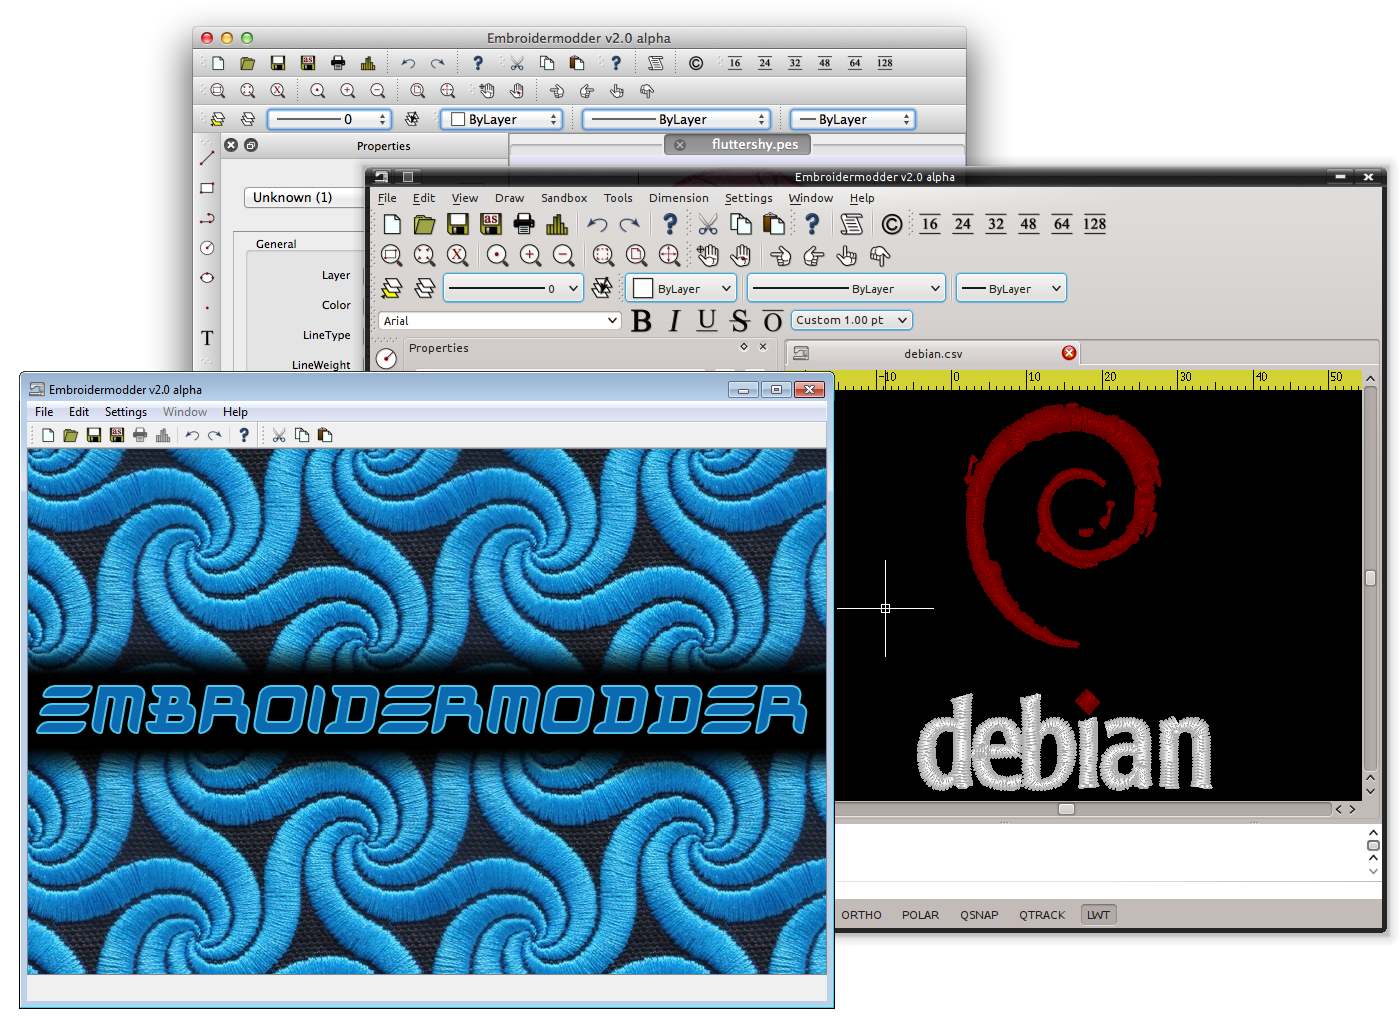
\includegraphics[width=0.9\textwidth]{images/features-platforms-1.png}
\end{center}

\subsection{Realistic Rendering}
% <a name="anchorRealRender"></a>

It is important to be able to visualize what a design will look like when stitched and our pseudo ``3D'' realistic rendering helps achieve this.

Realistic rendering sample \#1:

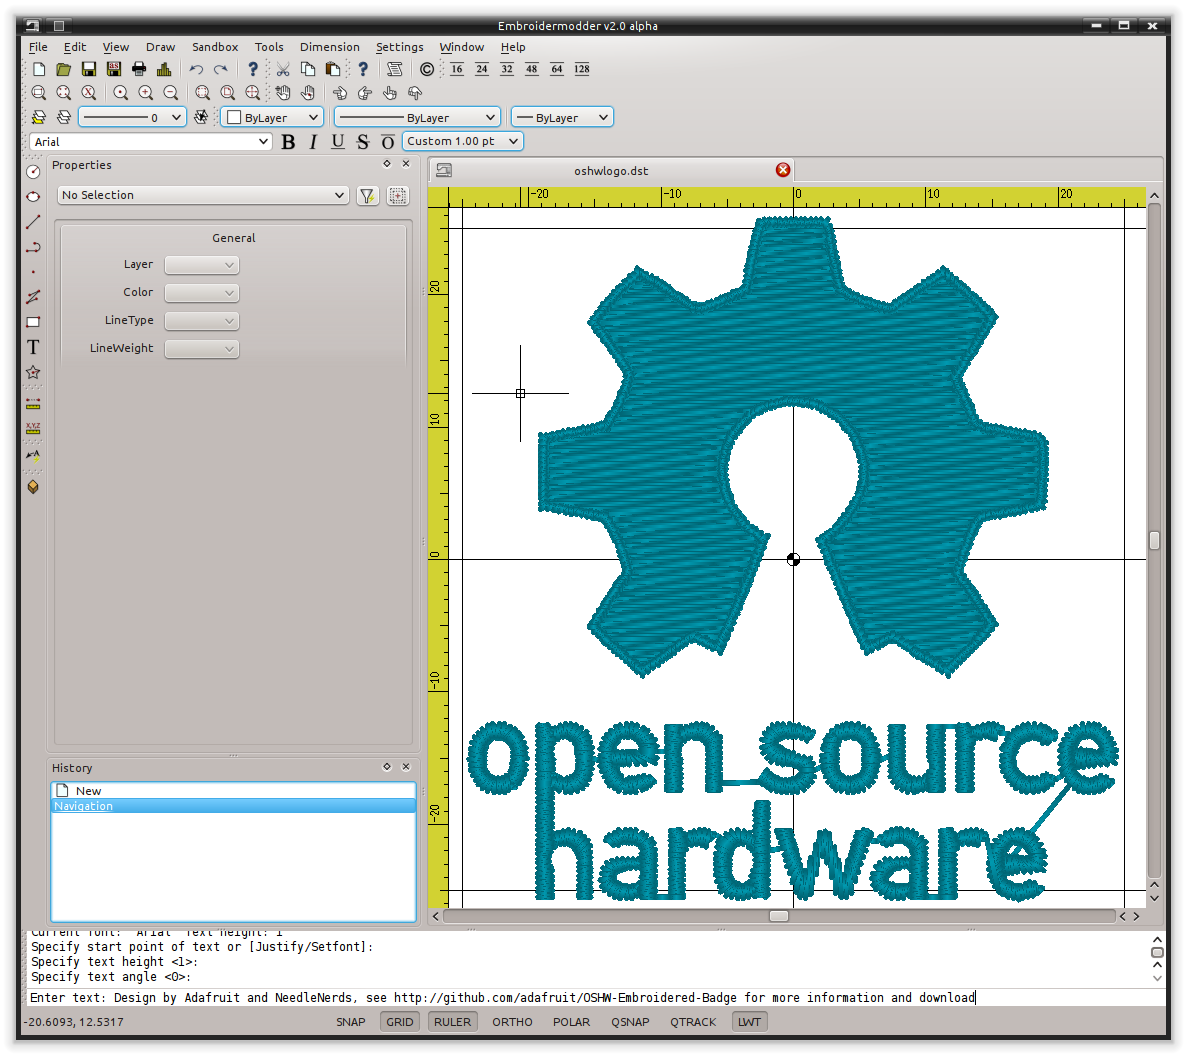
\includegraphics[width=0.9\textwidth]{images/features-realrender-1.png}

Realistic rendering sample \#2:

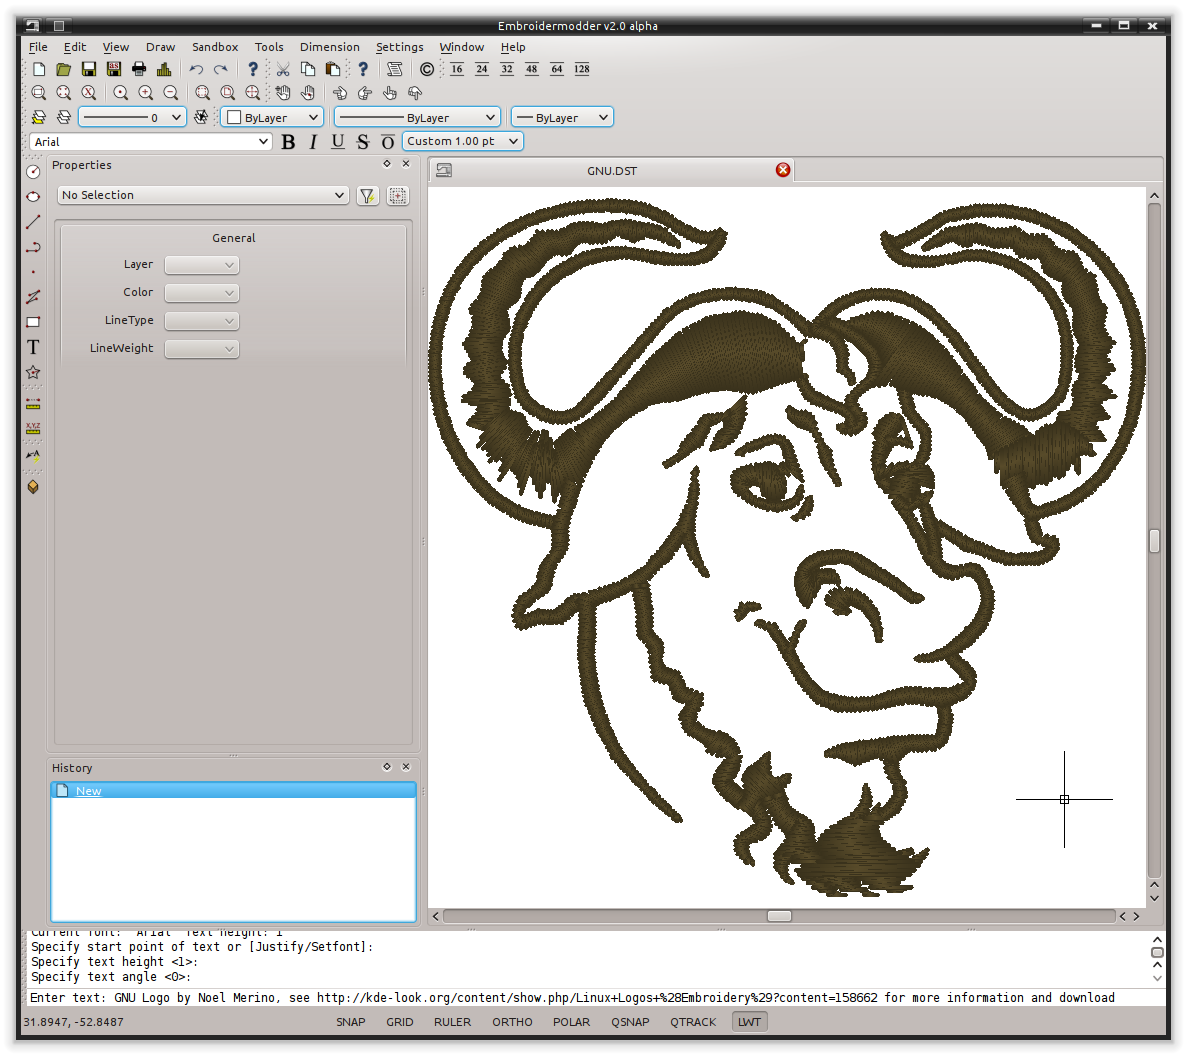
\includegraphics[width=0.9\textwidth]{images/features-realrender-2.png}

Realistic rendering sample \#3:

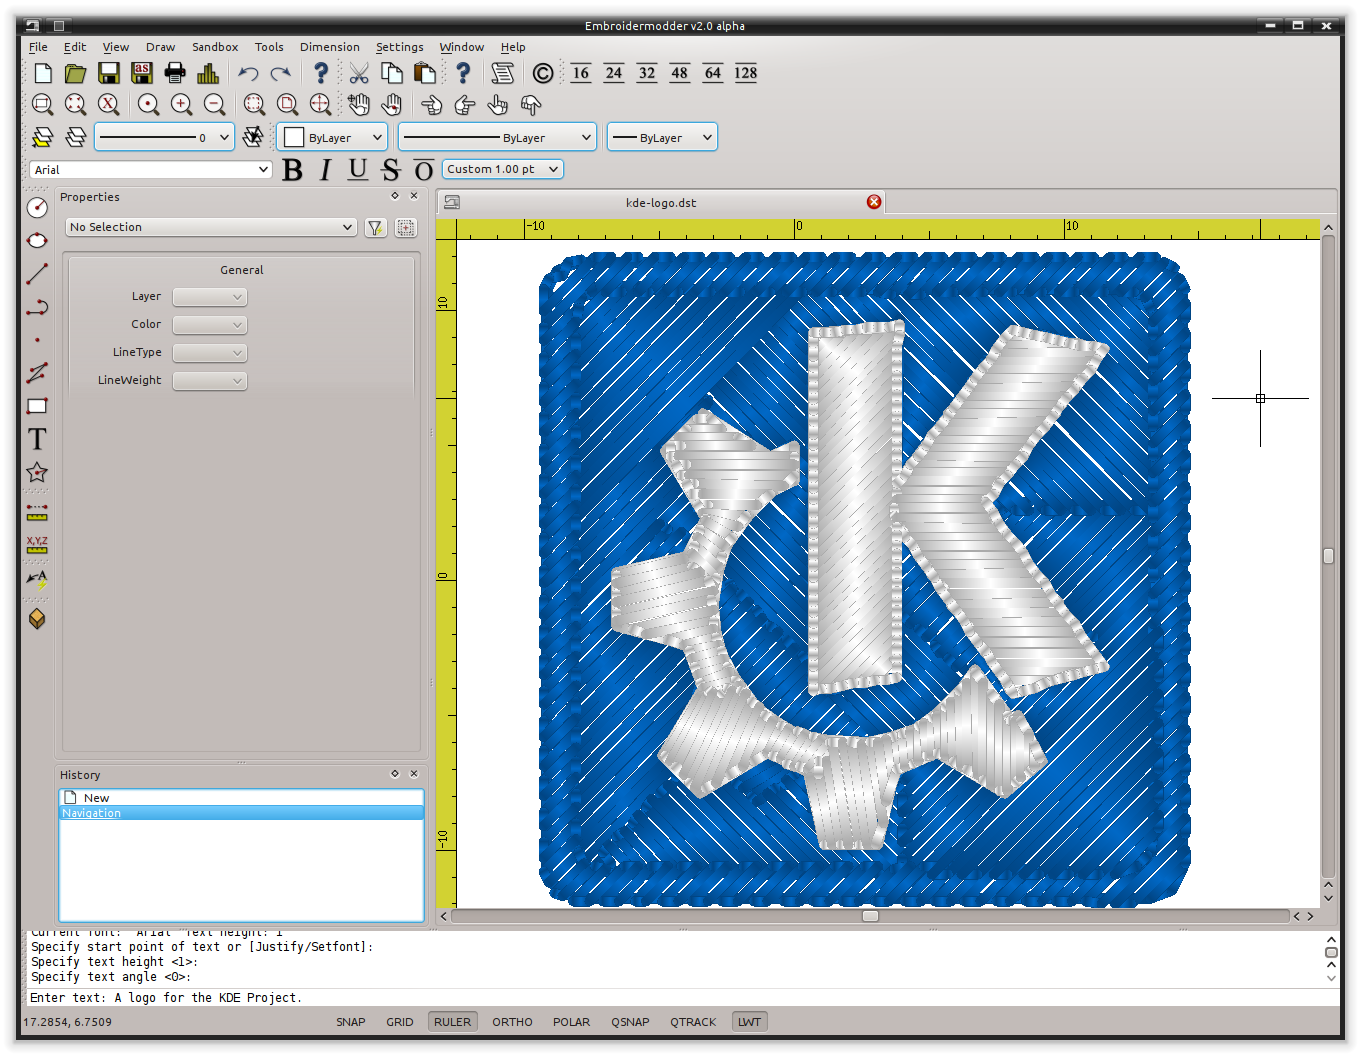
\includegraphics[width=0.9\textwidth]{images/features-realrender-3.png}

%<a name=``anchorGridRuler``></a>
Various grid types and auto-adjusting rulers

Making use of the automatically adjusting ruler in conjunction with the grid will ensure your design is properly sized and fits within your embroidery hoop area.

Use rectangular, circular or isometric grids to construct your masterpiece!

Multiple grids and rulers in action:

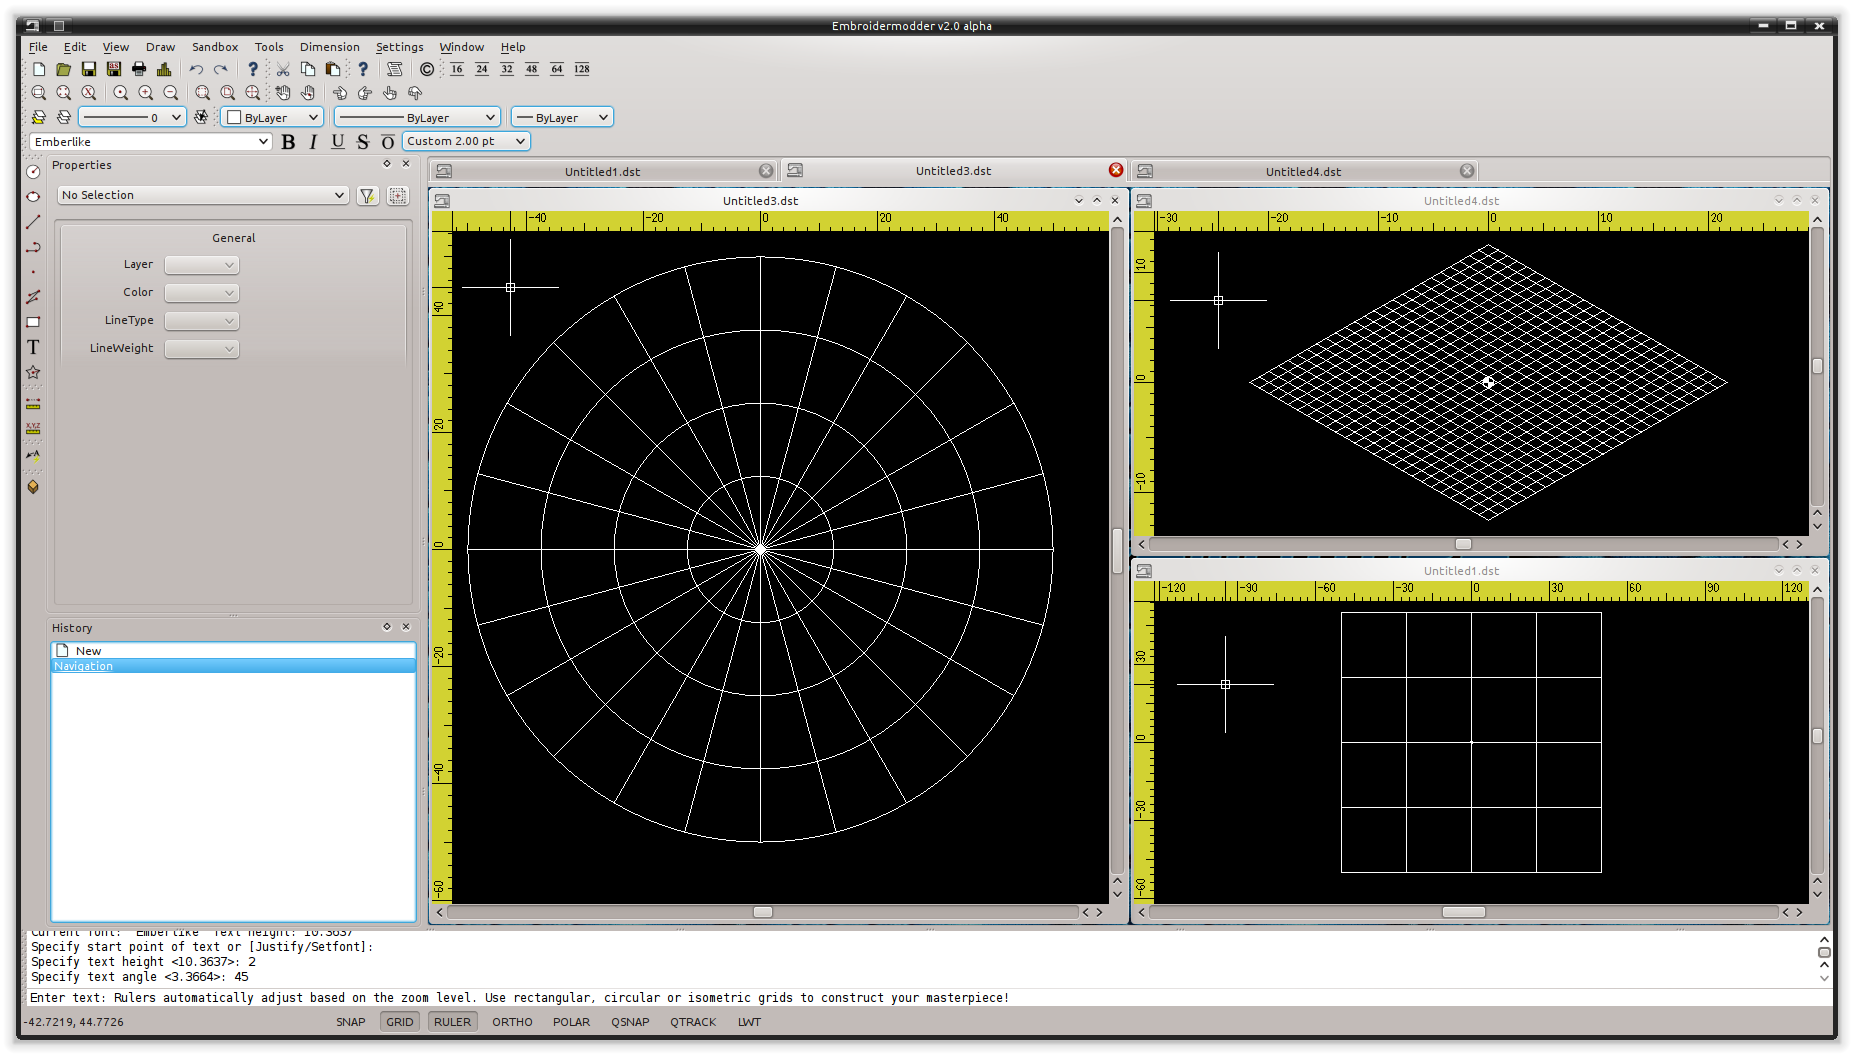
\includegraphics[width=0.9\textwidth]{images/features-grid-ruler-1.png}

\subsection{Many measurement tools}
%<a name="anchorMultiMeasure"></a>

Taking measurements is a critical part of creating great designs. Whether you are designing mission critical embroidered space suits for NASA or some other far out design for your next meet-up, you will have precise measurement tools at your command to make it happen. You can locate individual points or find distances between any 2 points anywhere in the design!

Take quick and accurate measurements:

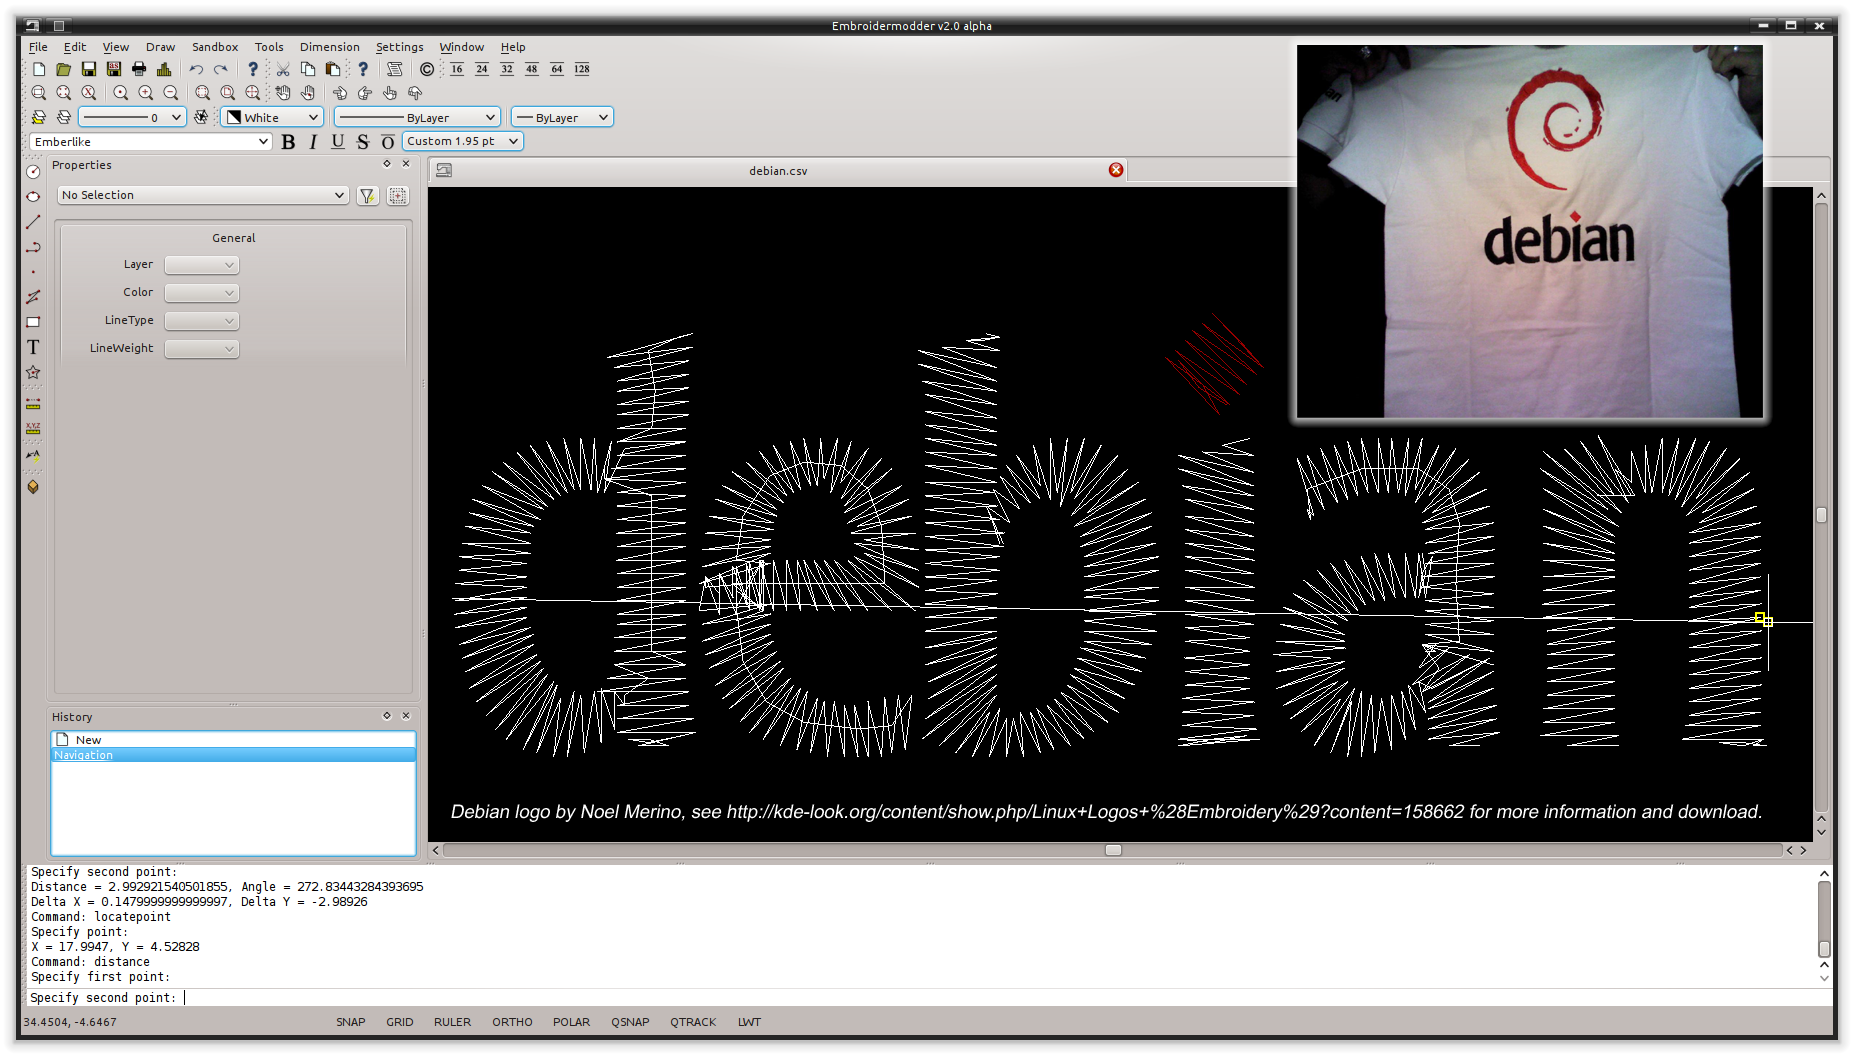
\includegraphics[width=0.9\textwidth]{images/features-measure-1.png}

\subsection{Add text to any design}
%<a name=``anchorText``></a>

Need to make company apparel for all of your employees with individual names on them? No sweat. Just simply add text to your existing design or create one from scratch, quickly and easily.
Didn't get it the right size or made a typo? No problem. Just select the text and update it with the property editor.

Add text and adjust its properties quickly:

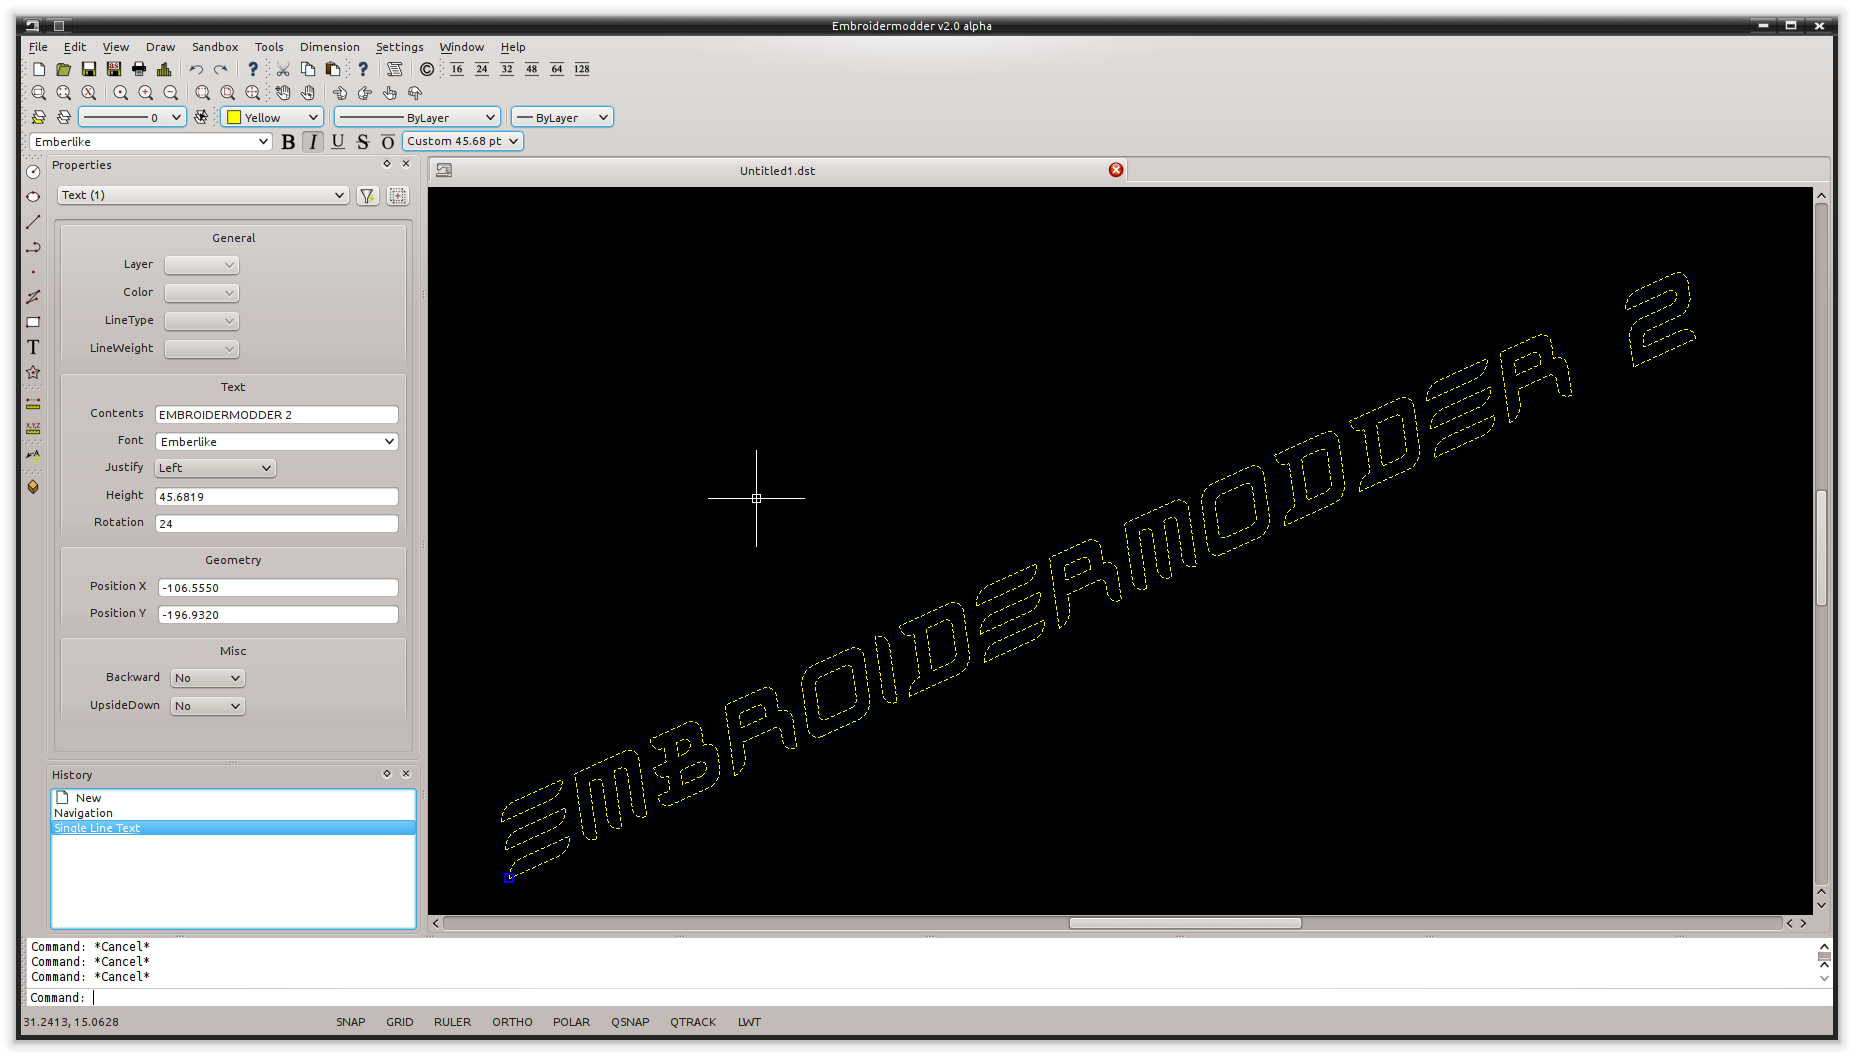
\includegraphics[width=0.9\textwidth]{images/features-text-1.png}

\subsection{Supports many formats}
%<a name="anchorFormats"></a>

Embroidery machines all accept different formats. There are so many formats available that it can sometimes be confusing whether a design will work with your machine.

Embroidermodder 2 supports a wide variety of embroidery formats as well as several vector formats, such as SVG and DXF. This allows you to worry less about which designs you can use.

\subsection{Batch Conversion}
%<a name=``anchorBatch``></a>

Need to send a client several different formats? Just use libembroidery-convert, our command line utility which supports batch file conversion.

There are a multitude of formats to choose from:

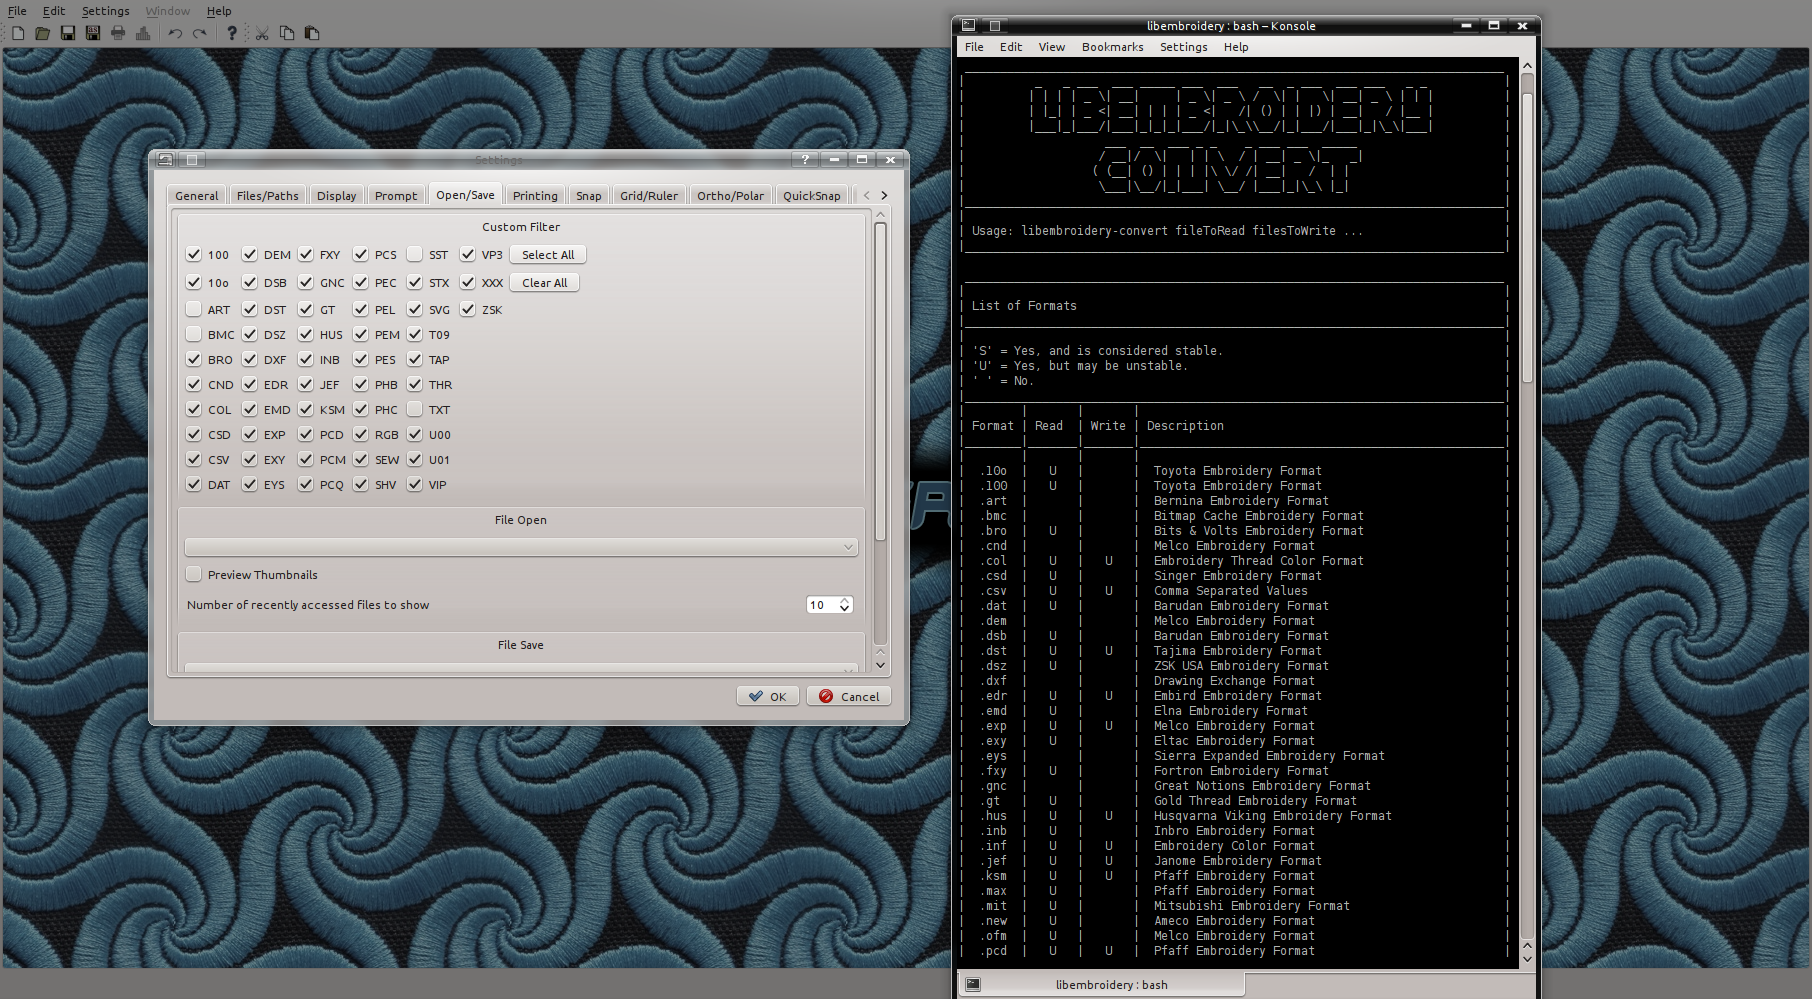
\includegraphics[width=0.9\textwidth]{images/features-formats-1.png}

\subsection{Scripting API}
%<a name=``anchorScriptingAPI``></a>

If you've got programming skills and there is a feature that isn't currently available that you absolutely cannot live without, you have the capability to create your own custom commands for Embroidermodder 2. We provide an QtScript API which exposes various application functionality so that it is possible to extend the application without requiring a new release. If you have created a command that you think is worth including in the next release, just <a href=``contact.html``>contact us</a> and we will review it for functionality, bugs, and finally inclusion.

An Embroidermodder 2 command excerpt:

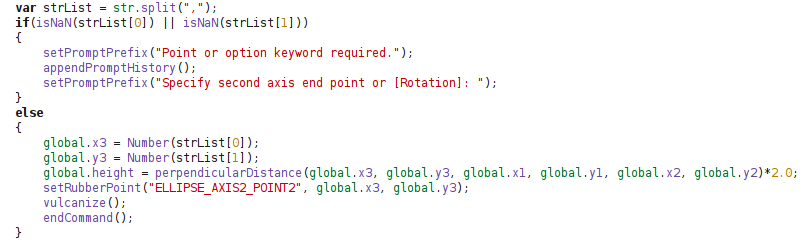
\includegraphics[width=0.9\textwidth]{images/features-scripting-1.png}

\section{Contributing}

\subsection{Version Control}

Being an open source project, developers can grab the latest code at any time
and attempt to build it themselves. We try our best to ensure that it will build smoothly
at any time, although occasionally we do break the build. In these instances,
please provide a patch, pull request which fixes the issue or open an issue and
notify us of the problem, as we may not be aware of it and we can build fine.

Try to group commits based on what they are related to: features/bugs/comments/graphics/commands/etc...

See the coding style [here](libembroidery\_style.md)

\section{Table of Contents}

  1. [Introduction](introduction)
  2. [Basic Features](basic-features)
  3. [Advanced Features](advanced-features)
  4. [Other Projects](other-projects)
  5. [References](References)

\section{Introduction}

\section{Basic Features}

\subsection{Move a single stitch in an existing pattern}

\begin{enumerate}
\item In the `File' menu, click `Open...'. When the open dialog appears find
  and select your file by double clicking the name of the file. Alternatively,
  left click the file once then click the `Open` button.
\item
\item In the `File' menu
\end{enumerate}

TIP: For users who prefer

\subsection{Convert one pattern to another format}

\begin{enumerate}
\item In the `File` menu, click `Open...`.
\item The 
\item In the dropdown menu within the save dialog select the 
\end{enumerate}

\section{Advanced Features}

\section{Other Projects}


\section{References}


\subsection{Planning}

To see what's planned open the [Projects](https://github.com/Embroidermodder/Embroidermodder/projects/1) tab which sorts all of the GitHub Issues into columns.

\subsection{Format Support}

\begin{tabular}{l l l l}
FORMAT & READ & WRITE & NOTES \\
\hline
10o    & YES   &       & read (need to fix external color loading) (maybe find out what ctrl\& code flags of 0x10, 0x08, 0x04, and 0x02 mean) \\
100    &       &       & none (4 byte codes) 61 00 10 09 (type, type2, x, y ?) x | y (signed char) \\
art    &       &       & none \\
bro    & YES   &       & read (complete)(maybe figure out detail of header) \\
cnd    &       &       & none \\
col    &       &       & (color file no design) read(final) write(final) \\
csd    & YES   &       & read (complete) \\
dat    &       &       & read () \\
dem    &       &       & none (looks like just encrypted cnd) \\
dsb    & YES   &       & read (unknown how well) (stitch data looks same as 10o) \\
dst    & YES   &       & read (complete) / write(unknown) \\
dsz    & YES   &       & read (unknown) \\
dxf    &       &       & read (Port to C. needs refactored) \\
edr    &       &       & read (C version is broken) / write (complete) \\
emd    &       &       & read (unknown) \\
exp    & YES   &       & read (unknown) / write(unknown) \\
exy    & YES   &       & read (need to fix external color loading) \\
fxy    & YES   &       & read (need to fix external color loading) \\
gnc    &       &       & none \\
gt     &       &       & read (need to fix external color loading) \\
hus    & YES   &       & read (unknown) / write (C version is broken) \\
inb    & YES   &       & read (buggy?) \\
jef    & YES   &       & write (need to fix the offsets when it is moving to another spot) \\
ksm    & YES   &       & read (unknown) / write (unknown) \\
pcd    &       &       &  \\
pcm    &       &       & \\
pcq    &       &       & read (Port to C)\\
pcs    & BUGGY &       & read (buggy / colors are not correct / after reading, writing any other format is messed up)\\
pec    &       &       & read / write (without embedded images, sometimes overlooks some stitches leaving a gap)\\
pel    &       &       & none\\
pem    &       &       & none\\
pes    & YES   &       & \\
phb    &       &       & \\
phc    &       &       & \\
rgb    &       &       & \\
sew    & YES   &       & \\
shv    &       &       & read (C version is broken)\\
sst    &       &       & none\\
svg    &       & YES   & \\
tap    & YES   &       & read (unknown)\\
u01    &       &       & \\
vip    & YES   &       & \\
vp3    & YES   &       & \\
xxx    & YES   &       & \\
zsk    &       &       & read (complete)
\end{tabular}

Support for Singer FHE, CHE (Compucon) formats?

\section{Embroidermodder Project Coding Standards}

A basic set of guidelines to use when submitting code.

\subsection{Naming Conventions}

Name variables and functions intelligently to minimize the need for comments.
It should be immediately obvious what information it represents.
Short names such as x and y are fine when referring to coordinates.
Short names such as i and j are fine when doing loops.

Variable names should be ``camelCase'', starting with a lowercase word followed by uppercase word(s).
C++ Class Names should be ``CamelCase'', using all uppercase word(s).
C Functions that attempt to simulate namespacing, should be ``nameSpace\_camelCase''.

All files and directories shall be lowercase and contain no spaces.

\section{Code Style}

Tabs should not be used when indenting. Setup your IDE or text editor to use 4 spaces.

\subsection{Braces}

For functions: please put each brace on a new line.

\begin{verbatim}
    void function_definition(int argument)
    {
    
    }
  \end{verbatim}

For control statements: please put the first brace on the same line.

\begin{verbatim}
    if (condition) {
    
    }
\end{verbatim}

Use exceptions sparingly.

Do not use ternary operator (?:) in place of if/else.

Do not repeat a variable name that already occurs in an outer scope.

\subsection{Version Control}

Being an open source project, developers can grab the latest code at any time
and attempt to build it themselves. We try our best to ensure that it will build smoothly
at any time, although occasionally we do break the build. In these instances,
please provide a patch, pull request which fixes the issue or open an issue and
notify us of the problem, as we may not be aware of it and we can build fine.

Try to group commits based on what they are related to: features/bugs/comments/graphics/commands/etc...

\subsection{Comments}

When writing code, sometimes there are items that we know can be improved,
incomplete or need special clarification. In these cases, use the types of
comments shown below. They are pretty standard and are highlighted by many editors to
make reviewing code easier. We also use shell scripts to parse the code to find
all of these occurrences so someone wanting to go on a bug hunt will be able to
easily see which areas of the code need more love. Use the same convention
as libembroidery.

libembroidery is written in C and adheres to C89 standards. This means
that any C99 or C++ comments will show up as errors when compiling with
gcc. In any C code, you must use:

\begin{verbatim}
    /* C Style Comments */

    /* TODO: This code clearly needs more work or further review. */

    /* BUG: This code is definitely wrong. It needs fixed. */

    /* HACK: This code shouldn't be written this way or I don't feel
     * right about it. There may a better solution */

    /* WARNING: Think twice (or more times) before changing this code.
     * I put this here for a good reason. */

    /* NOTE: This comment is much more important than lesser comments. */
\end{verbatim}

\subsection{Donations}

Creating software that interfaces with hardware is costly. A summary of some of the costs involved:
     
\begin{itemize}               
\item Developer time for 2 core developers
\item Computer equipment and parts
\item Embroidery machinery
\item Various electronics
\item Consumable materials (thread, fabric, stabilizer, etc...)
\end{itemize}

If you have found our software useful, please consider funding further development by donating to the project [on Open Collective](https://opencollective.com/embroidermodder).

\chapter{Mobile Support: MobileViewer and iMobileViewer}


\chapter{Conclusions}

\bibliographystyle{plainnat}
\bibliography{main.bib}

\appendix

% This is set up to run with pdflatex.
%---------The file header---------------------------------------------

\hfuzz = .6pt % avoid black boxes

%---------------------------------------------------------------------
\chapter*{\rlap{GNU Free Documentation License}}
\phantomsection  % so hyperref creates bookmarks
\addcontentsline{toc}{chapter}{GNU Free Documentation License}
%\label{label_fdl}

 \begin{center}

       Version 1.3, 3 November 2008


 Copyright \copyright{} 2000, 2001, 2002, 2007, 2008  Free Software Foundation, Inc.
 
 \bigskip
 
     \texttt{<https://fsf.org/>}
  
 \bigskip
 
 Everyone is permitted to copy and distribute verbatim copies
 of this license document, but changing it is not allowed.
\end{center}


\begin{center}
{\bf\large Preamble}
\end{center}

The purpose of this License is to make a manual, textbook, or other
functional and useful document ``free'' in the sense of freedom: to
assure everyone the effective freedom to copy and redistribute it,
with or without modifying it, either commercially or noncommercially.
Secondarily, this License preserves for the author and publisher a way
to get credit for their work, while not being considered responsible
for modifications made by others.

This License is a kind of ``copyleft'', which means that derivative
works of the document must themselves be free in the same sense.  It
complements the GNU General Public License, which is a copyleft
license designed for free software.

We have designed this License in order to use it for manuals for free
software, because free software needs free documentation: a free
program should come with manuals providing the same freedoms that the
software does.  But this License is not limited to software manuals;
it can be used for any textual work, regardless of subject matter or
whether it is published as a printed book.  We recommend this License
principally for works whose purpose is instruction or reference.


\begin{center}
{\Large\bf 1. APPLICABILITY AND DEFINITIONS\par}
\phantomsection
\addcontentsline{toc}{section}{1. APPLICABILITY AND DEFINITIONS}
\end{center}

This License applies to any manual or other work, in any medium, that
contains a notice placed by the copyright holder saying it can be
distributed under the terms of this License.  Such a notice grants a
world-wide, royalty-free license, unlimited in duration, to use that
work under the conditions stated herein.  The ``\textbf{Document}'', below,
refers to any such manual or work.  Any member of the public is a
licensee, and is addressed as ``\textbf{you}''.  You accept the license if you
copy, modify or distribute the work in a way requiring permission
under copyright law.

A ``\textbf{Modified Version}'' of the Document means any work containing the
Document or a portion of it, either copied verbatim, or with
modifications and/or translated into another language.

A ``\textbf{Secondary Section}'' is a named appendix or a front-matter section of
the Document that deals exclusively with the relationship of the
publishers or authors of the Document to the Document's overall subject
(or to related matters) and contains nothing that could fall directly
within that overall subject.  (Thus, if the Document is in part a
textbook of mathematics, a Secondary Section may not explain any
mathematics.)  The relationship could be a matter of historical
connection with the subject or with related matters, or of legal,
commercial, philosophical, ethical or political position regarding
them.

The ``\textbf{Invariant Sections}'' are certain Secondary Sections whose titles
are designated, as being those of Invariant Sections, in the notice
that says that the Document is released under this License.  If a
section does not fit the above definition of Secondary then it is not
allowed to be designated as Invariant.  The Document may contain zero
Invariant Sections.  If the Document does not identify any Invariant
Sections then there are none.

The ``\textbf{Cover Texts}'' are certain short passages of text that are listed,
as Front-Cover Texts or Back-Cover Texts, in the notice that says that
the Document is released under this License.  A Front-Cover Text may
be at most 5 words, and a Back-Cover Text may be at most 25 words.

A ``\textbf{Transparent}'' copy of the Document means a machine-readable copy,
represented in a format whose specification is available to the
general public, that is suitable for revising the document
straightforwardly with generic text editors or (for images composed of
pixels) generic paint programs or (for drawings) some widely available
drawing editor, and that is suitable for input to text formatters or
for automatic translation to a variety of formats suitable for input
to text formatters.  A copy made in an otherwise Transparent file
format whose markup, or absence of markup, has been arranged to thwart
or discourage subsequent modification by readers is not Transparent.
An image format is not Transparent if used for any substantial amount
of text.  A copy that is not ``Transparent'' is called ``\textbf{Opaque}''.

Examples of suitable formats for Transparent copies include plain
ASCII without markup, Texinfo input format, LaTeX input format, SGML
or XML using a publicly available DTD, and standard-conforming simple
HTML, PostScript or PDF designed for human modification.  Examples of
transparent image formats include PNG, XCF and JPG.  Opaque formats
include proprietary formats that can be read and edited only by
proprietary word processors, SGML or XML for which the DTD and/or
processing tools are not generally available, and the
machine-generated HTML, PostScript or PDF produced by some word
processors for output purposes only.

The ``\textbf{Title Page}'' means, for a printed book, the title page itself,
plus such following pages as are needed to hold, legibly, the material
this License requires to appear in the title page.  For works in
formats which do not have any title page as such, ``Title Page'' means
the text near the most prominent appearance of the work's title,
preceding the beginning of the body of the text.

The ``\textbf{publisher}'' means any person or entity that distributes
copies of the Document to the public.

A section ``\textbf{Entitled XYZ}'' means a named subunit of the Document whose
title either is precisely XYZ or contains XYZ in parentheses following
text that translates XYZ in another language.  (Here XYZ stands for a
specific section name mentioned below, such as ``\textbf{Acknowledgements}'',
``\textbf{Dedications}'', ``\textbf{Endorsements}'', or ``\textbf{History}''.)  
To ``\textbf{Preserve the Title}''
of such a section when you modify the Document means that it remains a
section ``Entitled XYZ'' according to this definition.

The Document may include Warranty Disclaimers next to the notice which
states that this License applies to the Document.  These Warranty
Disclaimers are considered to be included by reference in this
License, but only as regards disclaiming warranties: any other
implication that these Warranty Disclaimers may have is void and has
no effect on the meaning of this License.


\begin{center}
{\Large\bf 2. VERBATIM COPYING\par}
\phantomsection
\addcontentsline{toc}{section}{2. VERBATIM COPYING}
\end{center}

You may copy and distribute the Document in any medium, either
commercially or noncommercially, provided that this License, the
copyright notices, and the license notice saying this License applies
to the Document are reproduced in all copies, and that you add no other
conditions whatsoever to those of this License.  You may not use
technical measures to obstruct or control the reading or further
copying of the copies you make or distribute.  However, you may accept
compensation in exchange for copies.  If you distribute a large enough
number of copies you must also follow the conditions in section~3.

You may also lend copies, under the same conditions stated above, and
you may publicly display copies.


\begin{center}
{\Large\bf 3. COPYING IN QUANTITY\par}
\phantomsection
\addcontentsline{toc}{section}{3. COPYING IN QUANTITY}
\end{center}


If you publish printed copies (or copies in media that commonly have
printed covers) of the Document, numbering more than 100, and the
Document's license notice requires Cover Texts, you must enclose the
copies in covers that carry, clearly and legibly, all these Cover
Texts: Front-Cover Texts on the front cover, and Back-Cover Texts on
the back cover.  Both covers must also clearly and legibly identify
you as the publisher of these copies.  The front cover must present
the full title with all words of the title equally prominent and
visible.  You may add other material on the covers in addition.
Copying with changes limited to the covers, as long as they preserve
the title of the Document and satisfy these conditions, can be treated
as verbatim copying in other respects.

If the required texts for either cover are too voluminous to fit
legibly, you should put the first ones listed (as many as fit
reasonably) on the actual cover, and continue the rest onto adjacent
pages.

If you publish or distribute Opaque copies of the Document numbering
more than 100, you must either include a machine-readable Transparent
copy along with each Opaque copy, or state in or with each Opaque copy
a computer-network location from which the general network-using
public has access to download using public-standard network protocols
a complete Transparent copy of the Document, free of added material.
If you use the latter option, you must take reasonably prudent steps,
when you begin distribution of Opaque copies in quantity, to ensure
that this Transparent copy will remain thus accessible at the stated
location until at least one year after the last time you distribute an
Opaque copy (directly or through your agents or retailers) of that
edition to the public.

It is requested, but not required, that you contact the authors of the
Document well before redistributing any large number of copies, to give
them a chance to provide you with an updated version of the Document.


\begin{center}
{\Large\bf 4. MODIFICATIONS\par}
\phantomsection
\addcontentsline{toc}{section}{4. MODIFICATIONS}
\end{center}

You may copy and distribute a Modified Version of the Document under
the conditions of sections 2 and 3 above, provided that you release
the Modified Version under precisely this License, with the Modified
Version filling the role of the Document, thus licensing distribution
and modification of the Modified Version to whoever possesses a copy
of it.  In addition, you must do these things in the Modified Version:

\begin{itemize}
\item[A.] 
   Use in the Title Page (and on the covers, if any) a title distinct
   from that of the Document, and from those of previous versions
   (which should, if there were any, be listed in the History section
   of the Document).  You may use the same title as a previous version
   if the original publisher of that version gives permission.
   
\item[B.]
   List on the Title Page, as authors, one or more persons or entities
   responsible for authorship of the modifications in the Modified
   Version, together with at least five of the principal authors of the
   Document (all of its principal authors, if it has fewer than five),
   unless they release you from this requirement.
   
\item[C.]
   State on the Title page the name of the publisher of the
   Modified Version, as the publisher.
   
\item[D.]
   Preserve all the copyright notices of the Document.
   
\item[E.]
   Add an appropriate copyright notice for your modifications
   adjacent to the other copyright notices.
   
\item[F.]
   Include, immediately after the copyright notices, a license notice
   giving the public permission to use the Modified Version under the
   terms of this License, in the form shown in the Addendum below.
   
\item[G.]
   Preserve in that license notice the full lists of Invariant Sections
   and required Cover Texts given in the Document's license notice.
   
\item[H.]
   Include an unaltered copy of this License.
   
\item[I.]
   Preserve the section Entitled ``History'', Preserve its Title, and add
   to it an item stating at least the title, year, new authors, and
   publisher of the Modified Version as given on the Title Page.  If
   there is no section Entitled ``History'' in the Document, create one
   stating the title, year, authors, and publisher of the Document as
   given on its Title Page, then add an item describing the Modified
   Version as stated in the previous sentence.
   
\item[J.]
   Preserve the network location, if any, given in the Document for
   public access to a Transparent copy of the Document, and likewise
   the network locations given in the Document for previous versions
   it was based on.  These may be placed in the ``History'' section.
   You may omit a network location for a work that was published at
   least four years before the Document itself, or if the original
   publisher of the version it refers to gives permission.
   
\item[K.]
   For any section Entitled ``Acknowledgements'' or ``Dedications'',
   Preserve the Title of the section, and preserve in the section all
   the substance and tone of each of the contributor acknowledgements
   and/or dedications given therein.
   
\item[L.]
   Preserve all the Invariant Sections of the Document,
   unaltered in their text and in their titles.  Section numbers
   or the equivalent are not considered part of the section titles.
   
\item[M.]
   Delete any section Entitled ``Endorsements''.  Such a section
   may not be included in the Modified Version.
   
\item[N.]
   Do not retitle any existing section to be Entitled ``Endorsements''
   or to conflict in title with any Invariant Section.
   
\item[O.]
   Preserve any Warranty Disclaimers.
\end{itemize}

If the Modified Version includes new front-matter sections or
appendices that qualify as Secondary Sections and contain no material
copied from the Document, you may at your option designate some or all
of these sections as invariant.  To do this, add their titles to the
list of Invariant Sections in the Modified Version's license notice.
These titles must be distinct from any other section titles.

You may add a section Entitled ``Endorsements'', provided it contains
nothing but endorsements of your Modified Version by various
parties---for example, statements of peer review or that the text has
been approved by an organization as the authoritative definition of a
standard.

You may add a passage of up to five words as a Front-Cover Text, and a
passage of up to 25 words as a Back-Cover Text, to the end of the list
of Cover Texts in the Modified Version.  Only one passage of
Front-Cover Text and one of Back-Cover Text may be added by (or
through arrangements made by) any one entity.  If the Document already
includes a cover text for the same cover, previously added by you or
by arrangement made by the same entity you are acting on behalf of,
you may not add another; but you may replace the old one, on explicit
permission from the previous publisher that added the old one.

The author(s) and publisher(s) of the Document do not by this License
give permission to use their names for publicity for or to assert or
imply endorsement of any Modified Version.


\begin{center}
{\Large\bf 5. COMBINING DOCUMENTS\par}
\phantomsection
\addcontentsline{toc}{section}{5. COMBINING DOCUMENTS}
\end{center}


You may combine the Document with other documents released under this
License, under the terms defined in section~4 above for modified
versions, provided that you include in the combination all of the
Invariant Sections of all of the original documents, unmodified, and
list them all as Invariant Sections of your combined work in its
license notice, and that you preserve all their Warranty Disclaimers.

The combined work need only contain one copy of this License, and
multiple identical Invariant Sections may be replaced with a single
copy.  If there are multiple Invariant Sections with the same name but
different contents, make the title of each such section unique by
adding at the end of it, in parentheses, the name of the original
author or publisher of that section if known, or else a unique number.
Make the same adjustment to the section titles in the list of
Invariant Sections in the license notice of the combined work.

In the combination, you must combine any sections Entitled ``History''
in the various original documents, forming one section Entitled
``History''; likewise combine any sections Entitled ``Acknowledgements'',
and any sections Entitled ``Dedications''.  You must delete all sections
Entitled ``Endorsements''.

\begin{center}
{\Large\bf 6. COLLECTIONS OF DOCUMENTS\par}
\phantomsection
\addcontentsline{toc}{section}{6. COLLECTIONS OF DOCUMENTS}
\end{center}

You may make a collection consisting of the Document and other documents
released under this License, and replace the individual copies of this
License in the various documents with a single copy that is included in
the collection, provided that you follow the rules of this License for
verbatim copying of each of the documents in all other respects.

You may extract a single document from such a collection, and distribute
it individually under this License, provided you insert a copy of this
License into the extracted document, and follow this License in all
other respects regarding verbatim copying of that document.


\begin{center}
{\Large\bf 7. AGGREGATION WITH INDEPENDENT WORKS\par}
\phantomsection
\addcontentsline{toc}{section}{7. AGGREGATION WITH INDEPENDENT WORKS}
\end{center}


A compilation of the Document or its derivatives with other separate
and independent documents or works, in or on a volume of a storage or
distribution medium, is called an ``aggregate'' if the copyright
resulting from the compilation is not used to limit the legal rights
of the compilation's users beyond what the individual works permit.
When the Document is included in an aggregate, this License does not
apply to the other works in the aggregate which are not themselves
derivative works of the Document.

If the Cover Text requirement of section~3 is applicable to these
copies of the Document, then if the Document is less than one half of
the entire aggregate, the Document's Cover Texts may be placed on
covers that bracket the Document within the aggregate, or the
electronic equivalent of covers if the Document is in electronic form.
Otherwise they must appear on printed covers that bracket the whole
aggregate.


\begin{center}
{\Large\bf 8. TRANSLATION\par}
\phantomsection
\addcontentsline{toc}{section}{8. TRANSLATION}
\end{center}


Translation is considered a kind of modification, so you may
distribute translations of the Document under the terms of section~4.
Replacing Invariant Sections with translations requires special
permission from their copyright holders, but you may include
translations of some or all Invariant Sections in addition to the
original versions of these Invariant Sections.  You may include a
translation of this License, and all the license notices in the
Document, and any Warranty Disclaimers, provided that you also include
the original English version of this License and the original versions
of those notices and disclaimers.  In case of a disagreement between
the translation and the original version of this License or a notice
or disclaimer, the original version will prevail.

If a section in the Document is Entitled ``Acknowledgements'',
``Dedications'', or ``History'', the requirement (section~4) to Preserve
its Title (section~1) will typically require changing the actual
title.


\begin{center}
{\Large\bf 9. TERMINATION\par}
\phantomsection
\addcontentsline{toc}{section}{9. TERMINATION}
\end{center}


You may not copy, modify, sublicense, or distribute the Document
except as expressly provided under this License.  Any attempt
otherwise to copy, modify, sublicense, or distribute it is void, and
will automatically terminate your rights under this License.

However, if you cease all violation of this License, then your license
from a particular copyright holder is reinstated (a) provisionally,
unless and until the copyright holder explicitly and finally
terminates your license, and (b) permanently, if the copyright holder
fails to notify you of the violation by some reasonable means prior to
60 days after the cessation.

Moreover, your license from a particular copyright holder is
reinstated permanently if the copyright holder notifies you of the
violation by some reasonable means, this is the first time you have
received notice of violation of this License (for any work) from that
copyright holder, and you cure the violation prior to 30 days after
your receipt of the notice.

Termination of your rights under this section does not terminate the
licenses of parties who have received copies or rights from you under
this License.  If your rights have been terminated and not permanently
reinstated, receipt of a copy of some or all of the same material does
not give you any rights to use it.


\begin{center}
{\Large\bf 10. FUTURE REVISIONS OF THIS LICENSE\par}
\phantomsection
\addcontentsline{toc}{section}{10. FUTURE REVISIONS OF THIS LICENSE}
\end{center}


The Free Software Foundation may publish new, revised versions
of the GNU Free Documentation License from time to time.  Such new
versions will be similar in spirit to the present version, but may
differ in detail to address new problems or concerns.  See
\texttt{https://www.gnu.org/licenses/}.

Each version of the License is given a distinguishing version number.
If the Document specifies that a particular numbered version of this
License ``or any later version'' applies to it, you have the option of
following the terms and conditions either of that specified version or
of any later version that has been published (not as a draft) by the
Free Software Foundation.  If the Document does not specify a version
number of this License, you may choose any version ever published (not
as a draft) by the Free Software Foundation.  If the Document
specifies that a proxy can decide which future versions of this
License can be used, that proxy's public statement of acceptance of a
version permanently authorizes you to choose that version for the
Document.


\begin{center}
{\Large\bf 11. RELICENSING\par}
\phantomsection
\addcontentsline{toc}{section}{11. RELICENSING}
\end{center}


``Massive Multiauthor Collaboration Site'' (or ``MMC Site'') means any
World Wide Web server that publishes copyrightable works and also
provides prominent facilities for anybody to edit those works.  A
public wiki that anybody can edit is an example of such a server.  A
``Massive Multiauthor Collaboration'' (or ``MMC'') contained in the
site means any set of copyrightable works thus published on the MMC
site.

``CC-BY-SA'' means the Creative Commons Attribution-Share Alike 3.0
license published by Creative Commons Corporation, a not-for-profit
corporation with a principal place of business in San Francisco,
California, as well as future copyleft versions of that license
published by that same organization.

``Incorporate'' means to publish or republish a Document, in whole or
in part, as part of another Document.

An MMC is ``eligible for relicensing'' if it is licensed under this
License, and if all works that were first published under this License
somewhere other than this MMC, and subsequently incorporated in whole
or in part into the MMC, (1) had no cover texts or invariant sections,
and (2) were thus incorporated prior to November 1, 2008.

The operator of an MMC Site may republish an MMC contained in the site
under CC-BY-SA on the same site at any time before August 1, 2009,
provided the MMC is eligible for relicensing.


\begin{center}
{\Large\bf ADDENDUM: How to use this License for your documents\par}
\phantomsection
\addcontentsline{toc}{section}{ADDENDUM: How to use this License for your documents}
\end{center}

To use this License in a document you have written, include a copy of
the License in the document and put the following copyright and
license notices just after the title page:

\bigskip
\begin{quote}
    Copyright \copyright{}  YEAR  YOUR NAME.
    Permission is granted to copy, distribute and/or modify this document
    under the terms of the GNU Free Documentation License, Version 1.3
    or any later version published by the Free Software Foundation;
    with no Invariant Sections, no Front-Cover Texts, and no Back-Cover Texts.
    A copy of the license is included in the section entitled ``GNU
    Free Documentation License''.
\end{quote}
\bigskip
    
If you have Invariant Sections, Front-Cover Texts and Back-Cover Texts,
replace the ``with \dots\ Texts.''\ line with this:

\bigskip
\begin{quote}
    with the Invariant Sections being LIST THEIR TITLES, with the
    Front-Cover Texts being LIST, and with the Back-Cover Texts being LIST.
\end{quote}
\bigskip
    
If you have Invariant Sections without Cover Texts, or some other
combination of the three, merge those two alternatives to suit the
situation.

If your document contains nontrivial examples of program code, we
recommend releasing these examples in parallel under your choice of
free software license, such as the GNU General Public License,
to permit their use in free software.

%---------------------------------------------------------------------


\chapter{Color Charts}

\end{document}